

\newpage



%----------------------------------------------------------------------------------------


\section[Static Correlations][Corrélations Statiques]{Static correlations of urban form and network shape}{Corrélations Statiques entre Forme Urbaine et Forme de Réseau}

\label{sec:staticcorrelations}


%----------------------------------------------------------------------------------------



Une première entrée en matière empirique, et qui se voudra simple sur les objets étudiés, est de s'intéresser à des caractéristiques directement mesurables des territoires et réseaux. De manière phénoménologique, les agrégats urbains se qualifient au dessus d'une certaine échelle par une forme urbaine, de même que les réseaux de transport présentent des propriétés topologiques synthétiques. On peut alors s'interroger sur des liens directement mesurables entre ceux-ci, c'est à dire quelle information contiennent les corrélations statiques entre forme urbaine et topologie du réseau routier, au sens de corrélations estimées sur un échantillon local dans l'espace sur des données fixes. Dans une perspective de la Théorie Evolutive, on devine bien les implications de cette démarche: les liens entre corrélations dynamiques et statiques sont liées aux propriétés d'ergodicité du système, et la variation des estimateurs dans l'espace et selon les échelles informera sur le degré de stationnarité des interactions. Il s'agit d'une manière indirecte de lier statique et dynamique.


\comment{(Florent) c'est trop technique comme entrée en matière ; pourquoi faudrait il qu'il y ait de la diffusion ? et de quels processus parles tu ? la forme urbain / réseaux / les deux ?}

\bpar{
Spatio-temporal processes implying diffusion or propagation phenomena generally have a specific structure of correlation. In particular, as derived in section~\ref{sec:spatiotempcorrs}, a static computation of correlation between different instances of a system may under certain conditions provide information on dynamical correlations implied.
}{
Les processus spatio-temporels impliquant une diffusion ou une propagation peuvent généralement être compris partiellement par leur structure de correlation dans le temps et l'espace. On suggère par exemple en Appendice~\ref{sec:spatiotempcorrs} des cas idéaux pour lesquels un lien peut être directement obtenu. Dans certains cas, on peut espérer que l'étude d'une correlation statique entre différentes instances d'un système peuvent sous certaines conditions informer sur les correlations dynamiques sous-jacentes. Il s'agit typiquement de questions liées à l'ergodicité du système.
}




\bpar{
At the macroscopic scale of system of cities, the spatial nature of the urban system is reasonably captured by cities position, associated with aggregated city variable to represent entirely the system (see e.g. ontologies of Simpop models~\cite{pumain2012multi} or its successor Marius~\cite{cottineau2014evolution}). At the mesoscopic scale at which we aim to capture morphological manifestations of interactions between transportation networks and territories, structure of the territorial system can be specified by more refined indicators for the morphological aspect.
}{
A l'échelle macroscopique du système de ville, le caractère spatial du système urbain est capturé de manière raisonnable par les positions des villes, associées aux variables agrégées au niveau de la ville qui représentent entièrement le système, comme la plupart des modèles liés à la Théorie Evolutive postulent. A l'échelle mesoscopique, à laquelle nous nous attendons à capturer des manifestations morphologiques des interactions entre ville et transport, la structure du système territorial peut être spécifiée par des indicateurs plus raffinés pour l'aspect morphologique. Le choix des indicateurs de forme urbaine pertinents pour répondre à un type de question donnée n'est pas évident, et dépendra de l'échelle et du contexte : on peut par exemple s'intéresser au caractère polycentrique pour lequel les indicateurs seront différents si on s'intéresse à des phénomènes de concentration. Notre but est de capturer le maximum de dimensions de variation de la forme urbaine, nous calculerons pour cela un certain nombre d'indicateurs arbitraire satisfaisant une certaine convergence de la variance cumulée des composantes principales.
}



\bpar{
We study systematically morphological indicators for constant size areas covering a given geographical area. The choice of fixed size areas can be questioned regarding definition of a territorial system, that can be otherwise understood as a consistent spatial entity at a given scale and along certain criteria : \emph{Human territories} as defined by Raffestin (op. cit.) or more generally functionally autonomous spaces\footnote{for example, a tentative of definition of a \textit{Parisian} territory would present many facets. From the subjective territory point of view, intra-muros Parisians consider a strict boundary at \textit{Boulevard Periph{\'e}rique}, whereas close and even further suburbs will be seen as Parisians from the Province. The functional territory of \textit{Metropolitain} extends slightly further than the administrative boundary. Governance perimeters are currently mutating with the Metropolitan governance project. Complementary perceptions of the territory can thus be multiplied.}. Here we choose the mesoscopic scale of a metropolitan center ($\simeq$ 50km) for comparability purposes and because greater scale are no more relevant regarding urban form, whereas smaller scales must contain too much noise. 
}{
Nous étudions de manière systématique les indicateurs morphologiques pour des zones d'aire constante couvrant une région donnée. Le choix de zones de taille fixe peut être interrogé au regard de la définition d'un système territorial, qui peut par ailleurs être compris comme une entité spatiale consistante à une échelle donnée et selon certains critères : les \emph{Territoires Humains} comme nous avons déjà défini en~\ref{sec:thematic} ou plus généralement des espace fonctionnels autonomes\footnote{par example, tenter de définir un territoire \emph{Parisien} présenterait plusieurs facettes. Du point de vue du territoire subjectif, les Parisiens intra-muros considèrent une barrière stricte au Boulevard Périphérique, tandis que des banlieues plus ou moins proches seront vues comme parisiennes depuis la province. Le territoire fonctionnel du Métropolitain s'étend légèrement plus loin que la limite administrative de Paris, mais couvre quasiment toute l'Ile-de-France lorsqu'on y ajoute RER et Transilien. Les périmètres de gouvernance sont en train d'évoluer avec le projet de gouvernance métropolitaine (voir~\ref{sec:casestudies}). Des perceptions complémentaires du territoires peuvent ainsi être multipliées.}. Le choix de limites ``pertinentes'' pour le territoire ou la ville est un problème relativement ouvert \cite{guerois2002commune} qui dépendra souvent de la question à laquelle on cherche à répondre. Nous choisissons ici l'échelle mesoscopique d'un centre métropolitain ($\simeq$ 50km) d'une part pour la cohérence du champ spatial calculé, et d'autre part parce que des échelles plus grandes deviennent moins pertinentes pour la notion de forme urbaine, tandis que des échelles plus petites contiennent un bruit trop grand.
}


Le but n'étant pas de comparer les territoires sur lesquels ces indicateurs sont calculés entre eux, mais de calculer une valeur ``locale'' et d'établir un champ discret régulier dans l'espace, la taille fixe de la fenêtre est nécessaire. Cette taille est arbitraire, mais l'analyse a été menée pour des tailles voisines également (voir~\ref{app:sec:staticcorrelations}). Les ``territoires'' qu'une approche plus classique voudra comparer, comme des aires urbaines fonctionnelles par exemple, pourront émerger de manière endogène si ceux-ci font sens pour les variations des indicateurs.





%%%%%%%%%%%%%%%%%%
\subsection{Morphological Measures}{Mesures morphologiques}

\paragraph{Urban Morphology}{Morphologie Urbaine}


\bpar{
\cite{guerois2008built} studies the form of European cities using a simple measure of density slopes from the center to the periphery. We need however quantities having a certain level of robustness and invariance. For example, two polycentric cities should be classified as morphologically close whereas a direct comparison of distributions (with the Earth Mover Distance for example) could give a very high distance between configurations depending on center positions. The use of fractal indexes is a possibility suggested by~\cite{2016arXiv160808839C}. We choose to refer to the literature in Urban Morphology which proposes an extensive set of indicators to describe urban form~\cite{tsai2005quantifying}. The number of dimensions can be reduced to obtain a robust description with a few number of independent indicators~\cite{Schwarz201029}. Note that here we consider indicators on population density only, and that more elaborated considerations on Urban Form include for example the distribution of economic opportunities and the combination of these two fields through accessibility measures. For the choice of indicators, we follow the analysis done in~\cite{le2015forme} in which a morphological typology of large european cities is obtained.
}{
\cite{guerois2008built} étudie la forme des villes Européennes par l'utilisation d'une mesure simple des gradients de densité du centre vers la périphérie. Nous avons cependant besoin de mesures ayant un certain niveau de robustesse et d'invariance. Par exemple, deux villes polycentriques devraient être classifiées comme morphologiquement proches tandis qu'une comparaison directe des distributions (avec une distance de Monge par exemple) pourra donner une distance très élevée entre les configurations selon la position des centres. L'utilisation d'indices issus de l'analyse fractale est une possibilité suggérée par~\cite{2016arXiv160808839C}. Le lien entre morphologie urbaine et topologie du graphe de relations correspondant a été suggéré par\cite{badariotti2007conception}. Nous choisissons de nous référer à la littérature en morphologie urbaine qui propose des jeux d'indicateurs variés pour décrire la forme urbaine~\cite{tsai2005quantifying}. Le nombre de dimensions peut être réduit pour obtenir une description robuste avec un petit nombre d'indicateurs indépendants~\cite{Schwarz201029}. Il faut noter que nous ne considérons ici des indicateurs sur la densité de population seule, et que des considérations plus élaborées sur la forme urbaine incluent par exemple la distribution des opportunités économiques et la combinaison de ces deux champs par des mesures d'accessibilité. Pour le choix des indicateurs, nous suivons l'analyse faite dans~\cite{le2015forme} où une typologie morphologique des grandes villes européennes est obtenue.
}

\bpar{
We give now the formal definition of morphological indicators. We consider gridded population data $(P_i)_{1\leq i \leq N^2}$, write $M=N^2$ the number of cells, $d_{ij}$ the distance between cells $i,j$, and $P=\sum_{i=1}^{M} P_i$ total population. We measure Urban Form using:

\begin{enumerate}
\item Rank-size slope $\gamma$, expressing the degree of hierarchy in the distribution, computed by fitting with Ordinary Least Squares a power law distribution by $\ln \left( P_{\tilde{i}}/P_0\right) \sim k + \gamma\cdot \ln \left(\tilde{i}/i_0\right)$ where $\tilde{i}$ are the indexes of the distribution sorted in decreasing order. It is always negative, and values close to zero mean a flat distribution.
\item Entropy of the distribution, that expresses how uniform the distribution is:
\begin{equation}
\mathcal{E} = \sum_{i=1}^{M}\frac{P_i}{P}\cdot \ln{\frac{P_i}{P}}
\end{equation}
$\mathcal{E}=0$ means that all the population is in one cell whereas $\mathcal{E}=0$ means that the population is uniformly distributed.
\item Spatial-autocorrelation given by Moran index, with simple spatial weights given by $w_{ij} = 1/d_{ij}$
\[
I = \frac{\sum_{i\neq j} w_{ij} \left(P_i - \bar{P}\right)\cdot\left(P_j - \bar{P}\right)}{\sum_{i\neq j} w_{ij} \sum_{i}{\left( P_i - \bar{P}\right)}^2}
\]
Positive values will imply aggregation spots (``density centers''), negative values strong local variations whereas $I=0$ corresponds to totally random population values.
\item Mean distance between individuals, which captures population concentration
\[
\bar{d} = \frac{1}{d_M}\cdot \sum_{i<j} \frac{P_i P_j}{P^2} \cdot d_{ij}
\]
where $d_M$ is a normalisation constant taken as the diagonal of the world in our case.
\end{enumerate}
}{
Nous donnons à présent une définition formelle des indicateurs morphologiques. Nous considérons des données de population en grille $(P_i)_{1\leq i \leq N^2}$, écrivons $M=N^2$ le nombre de cellules, $d_{ij}$ la distance entre les cellules $i,j$, et $P=\sum_{i=1}^{M} P_i$ la population totale. La forme urbaine est mesurée par : 

\begin{enumerate}
\item Pente de la loi rang-taille $\gamma$, qui exprime le degré de hiérarchie de la distribution, calculé en ajustant une loi de puissance par Moindres Carrés Ordinaires par $\ln \left( P_{\tilde{i}}/P_0\right) \sim k + \gamma\cdot \ln \left(\tilde{i}/i_0\right)$ où $\tilde{i}$ sont les indices de la distribution triée de manière décroissante. Elle est toujours négative, et des valeurs proches de zéro signifient une distribution plate.
\item Entropie de la distribution, qui exprime l'uniformité de la distribution:
\begin{equation}
\mathcal{E} = \sum_{i=1}^{M}\frac{P_i}{P}\cdot \ln{\frac{P_i}{P}}
\end{equation}
$\mathcal{E}=0$ signifie que toute la population est dans une cellule tandis que $\mathcal{E}=0$ signifie que la population est distribuée uniformément.
\item L'auto-corrélation spatiale donnée par l'indice de Moran, avec des poids spatiaux simples donnés par $w_{ij} = 1/d_{ij}$
\[
I = \frac{\sum_{i\neq j} w_{ij} \left(P_i - \bar{P}\right)\cdot\left(P_j - \bar{P}\right)}{\sum_{i\neq j} w_{ij} \sum_{i}{\left( P_i - \bar{P}\right)}^2}
\]
Des valeurs positives impliques des lieux d'agrégation (``centres de densité''), des valeurs négatives des fortes variations locales, tandis que $I=0$ correspond à des valeurs de population totalement aléatoires.
\item Distance moyenne entre individus, qui capture la concentration de la population
\[
\bar{d} = \frac{1}{d_M}\cdot \sum_{i<j} \frac{P_i P_j}{P^2} \cdot d_{ij}
\]
où $d_M$ est une constante de normalisation que nous prenons comme la diagonale de l'étendue considérée dans notre cas.
\end{enumerate}
}

Les deux premiers indexes ne sont pas spatiaux, mais nécessaires pour une bonne qualification des distributions de population, et sont complétés par les deux derniers prenant en compte l'espace.


%%%%%%%%%%%%%%%%%%%%%%%%
\paragraph{Results}{Résultats}



%%%%%%%%%%%%%%%%%%%%%%%%
\begin{figure}
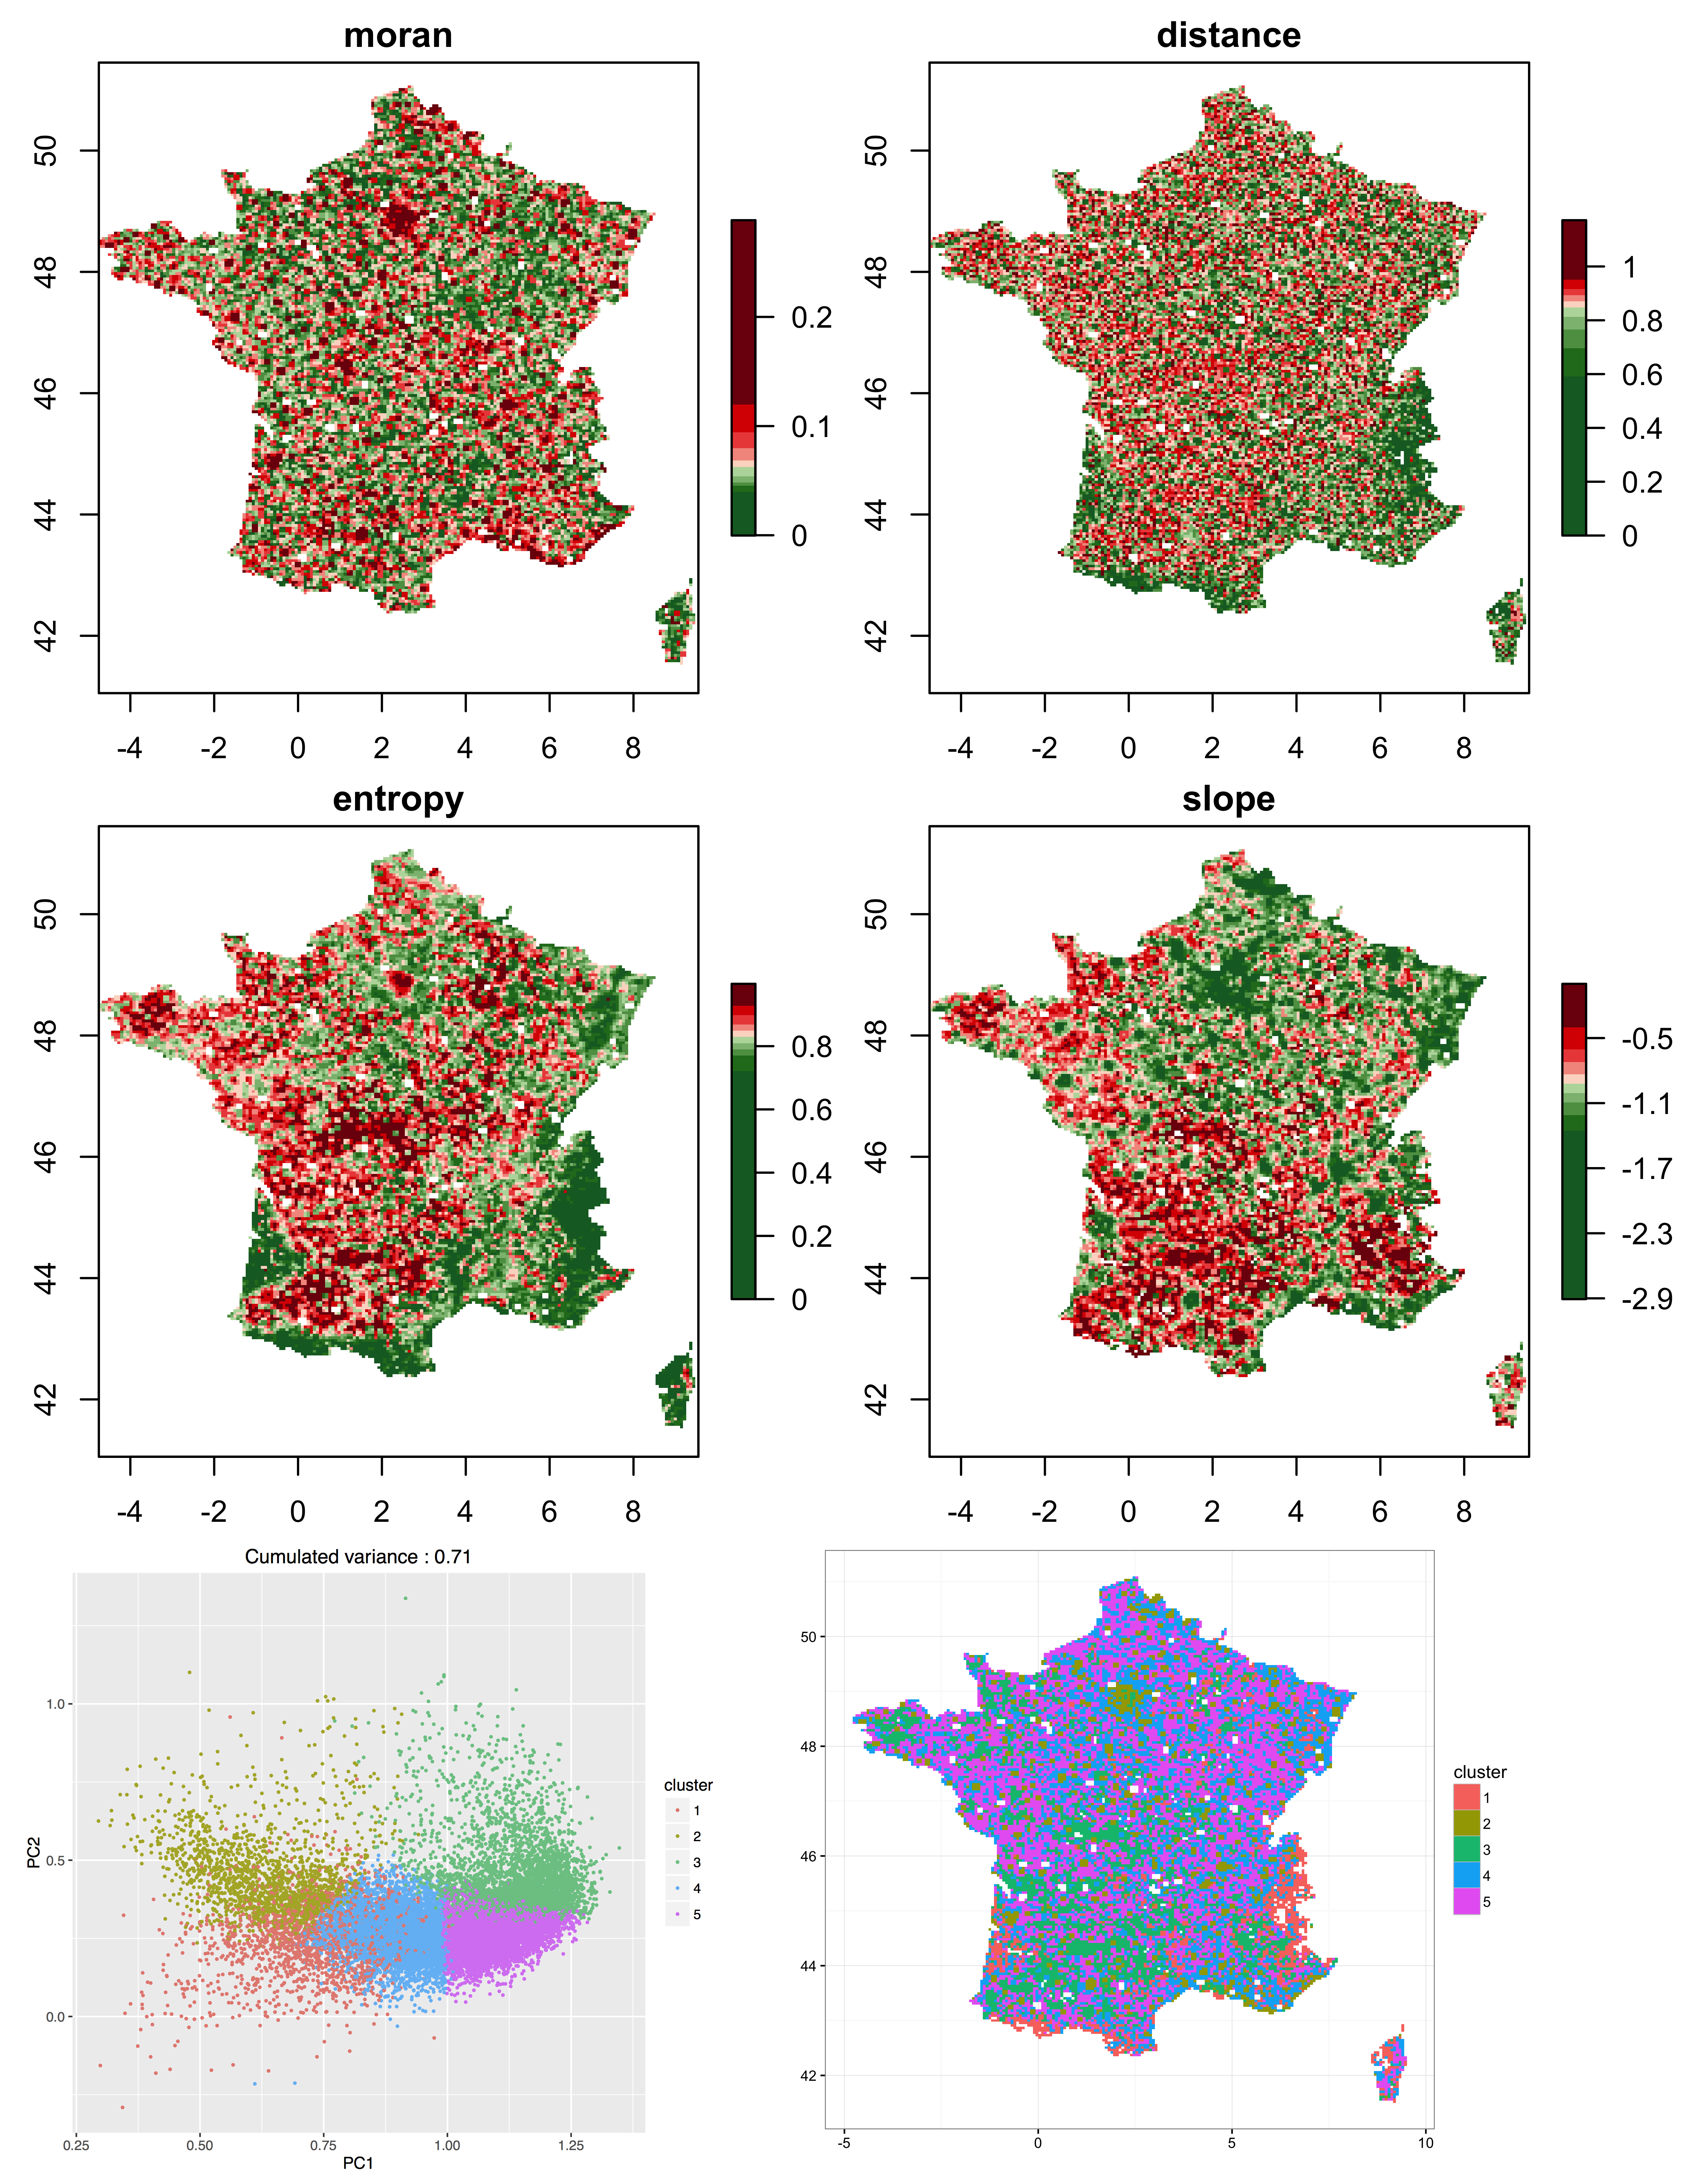
\includegraphics[width=0.9\linewidth]{Figures/Density/Fig1}
%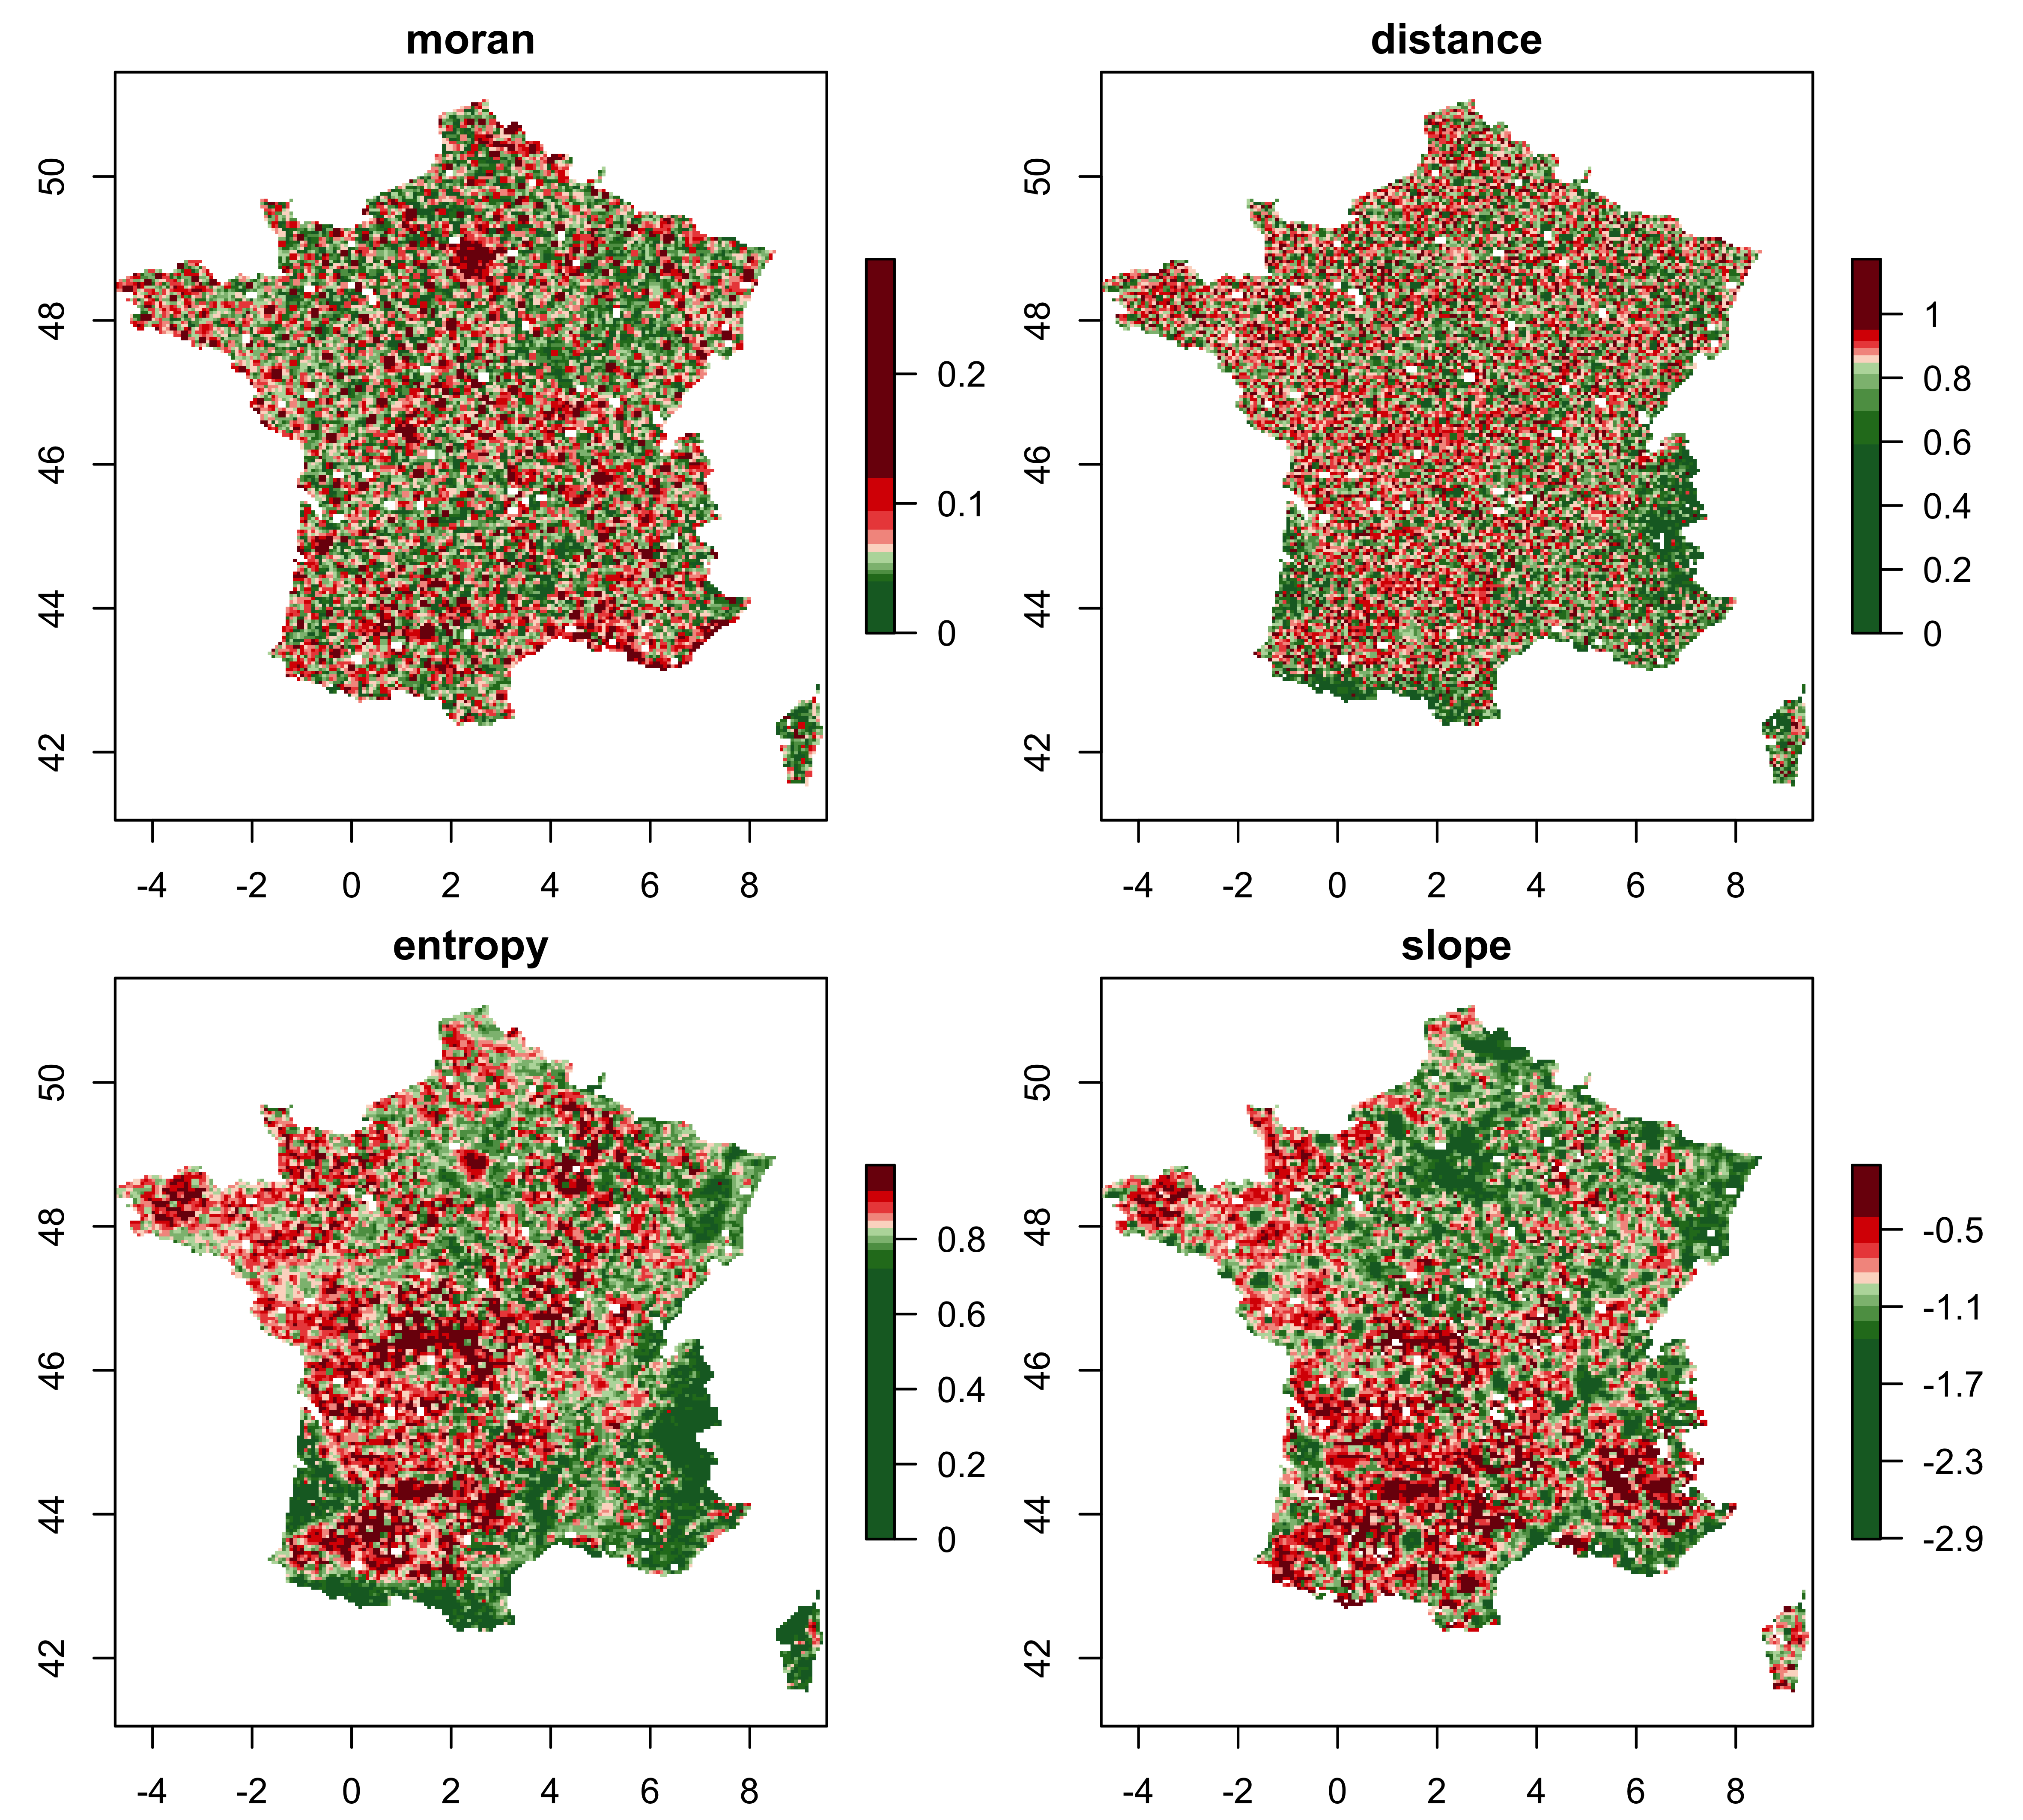
\includegraphics[width=\textwidth]{figures/indics_morpho_discrquantiles}\\
%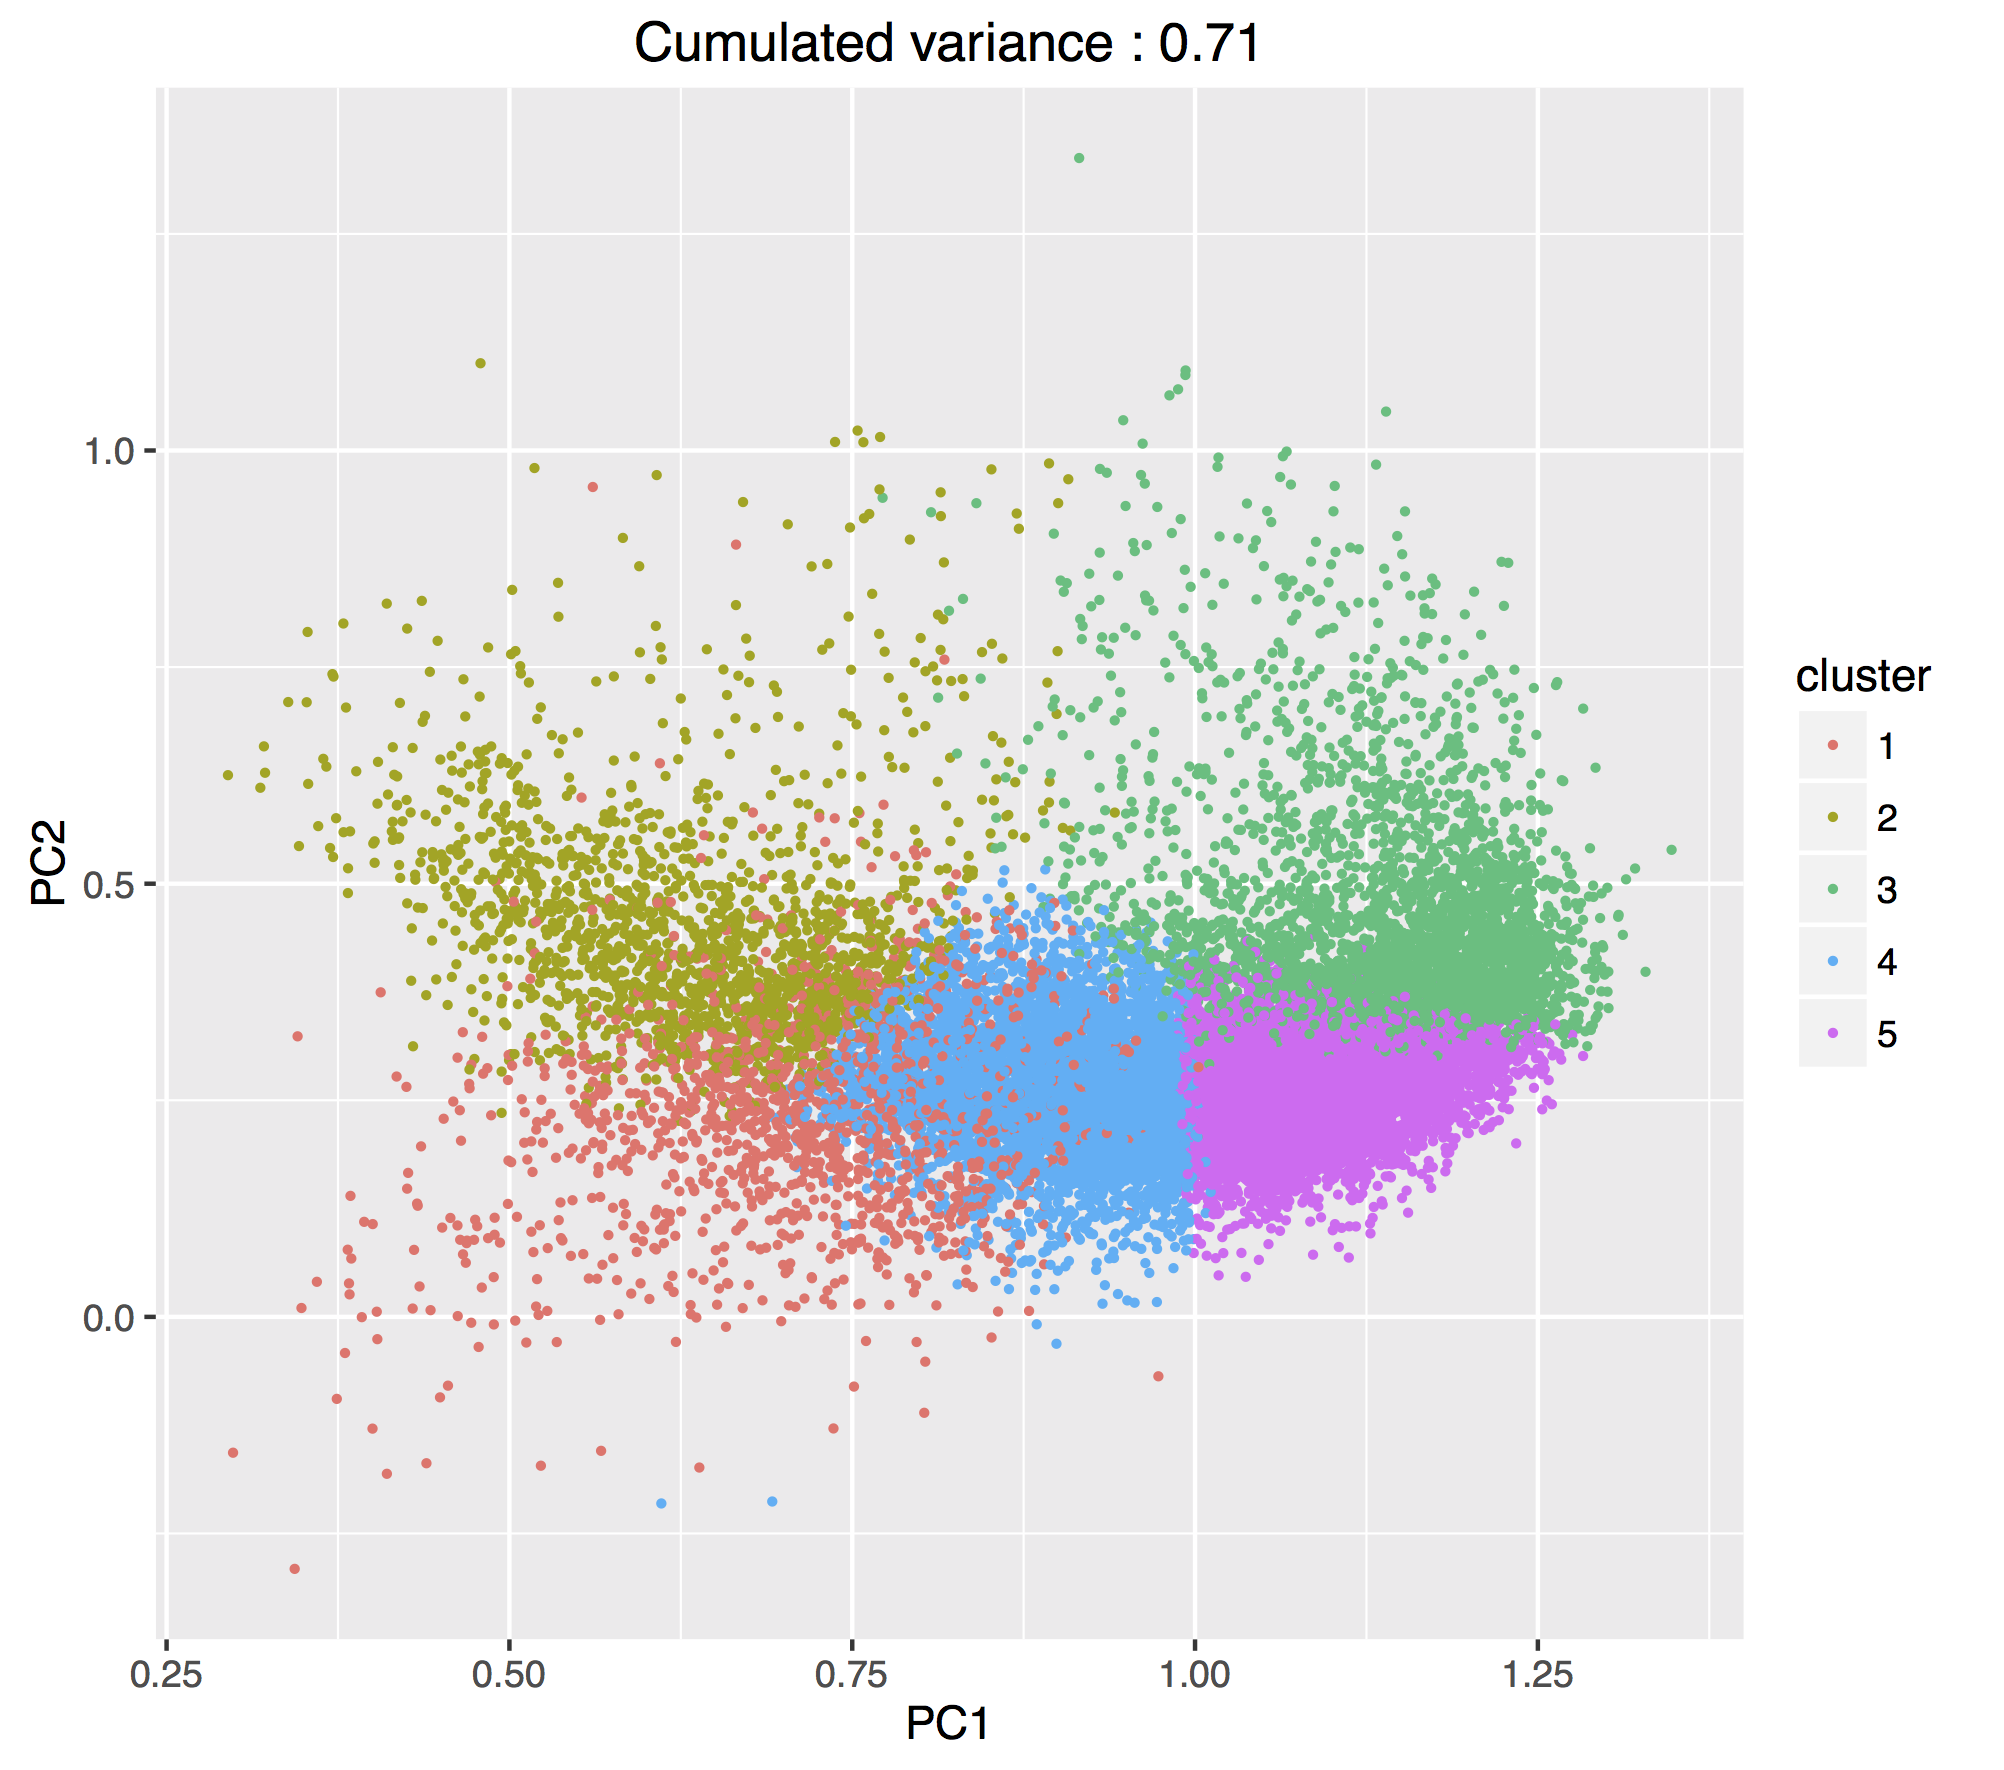
\includegraphics[width=0.49\textwidth]{figures/cluster_pca_k5_morpho}
%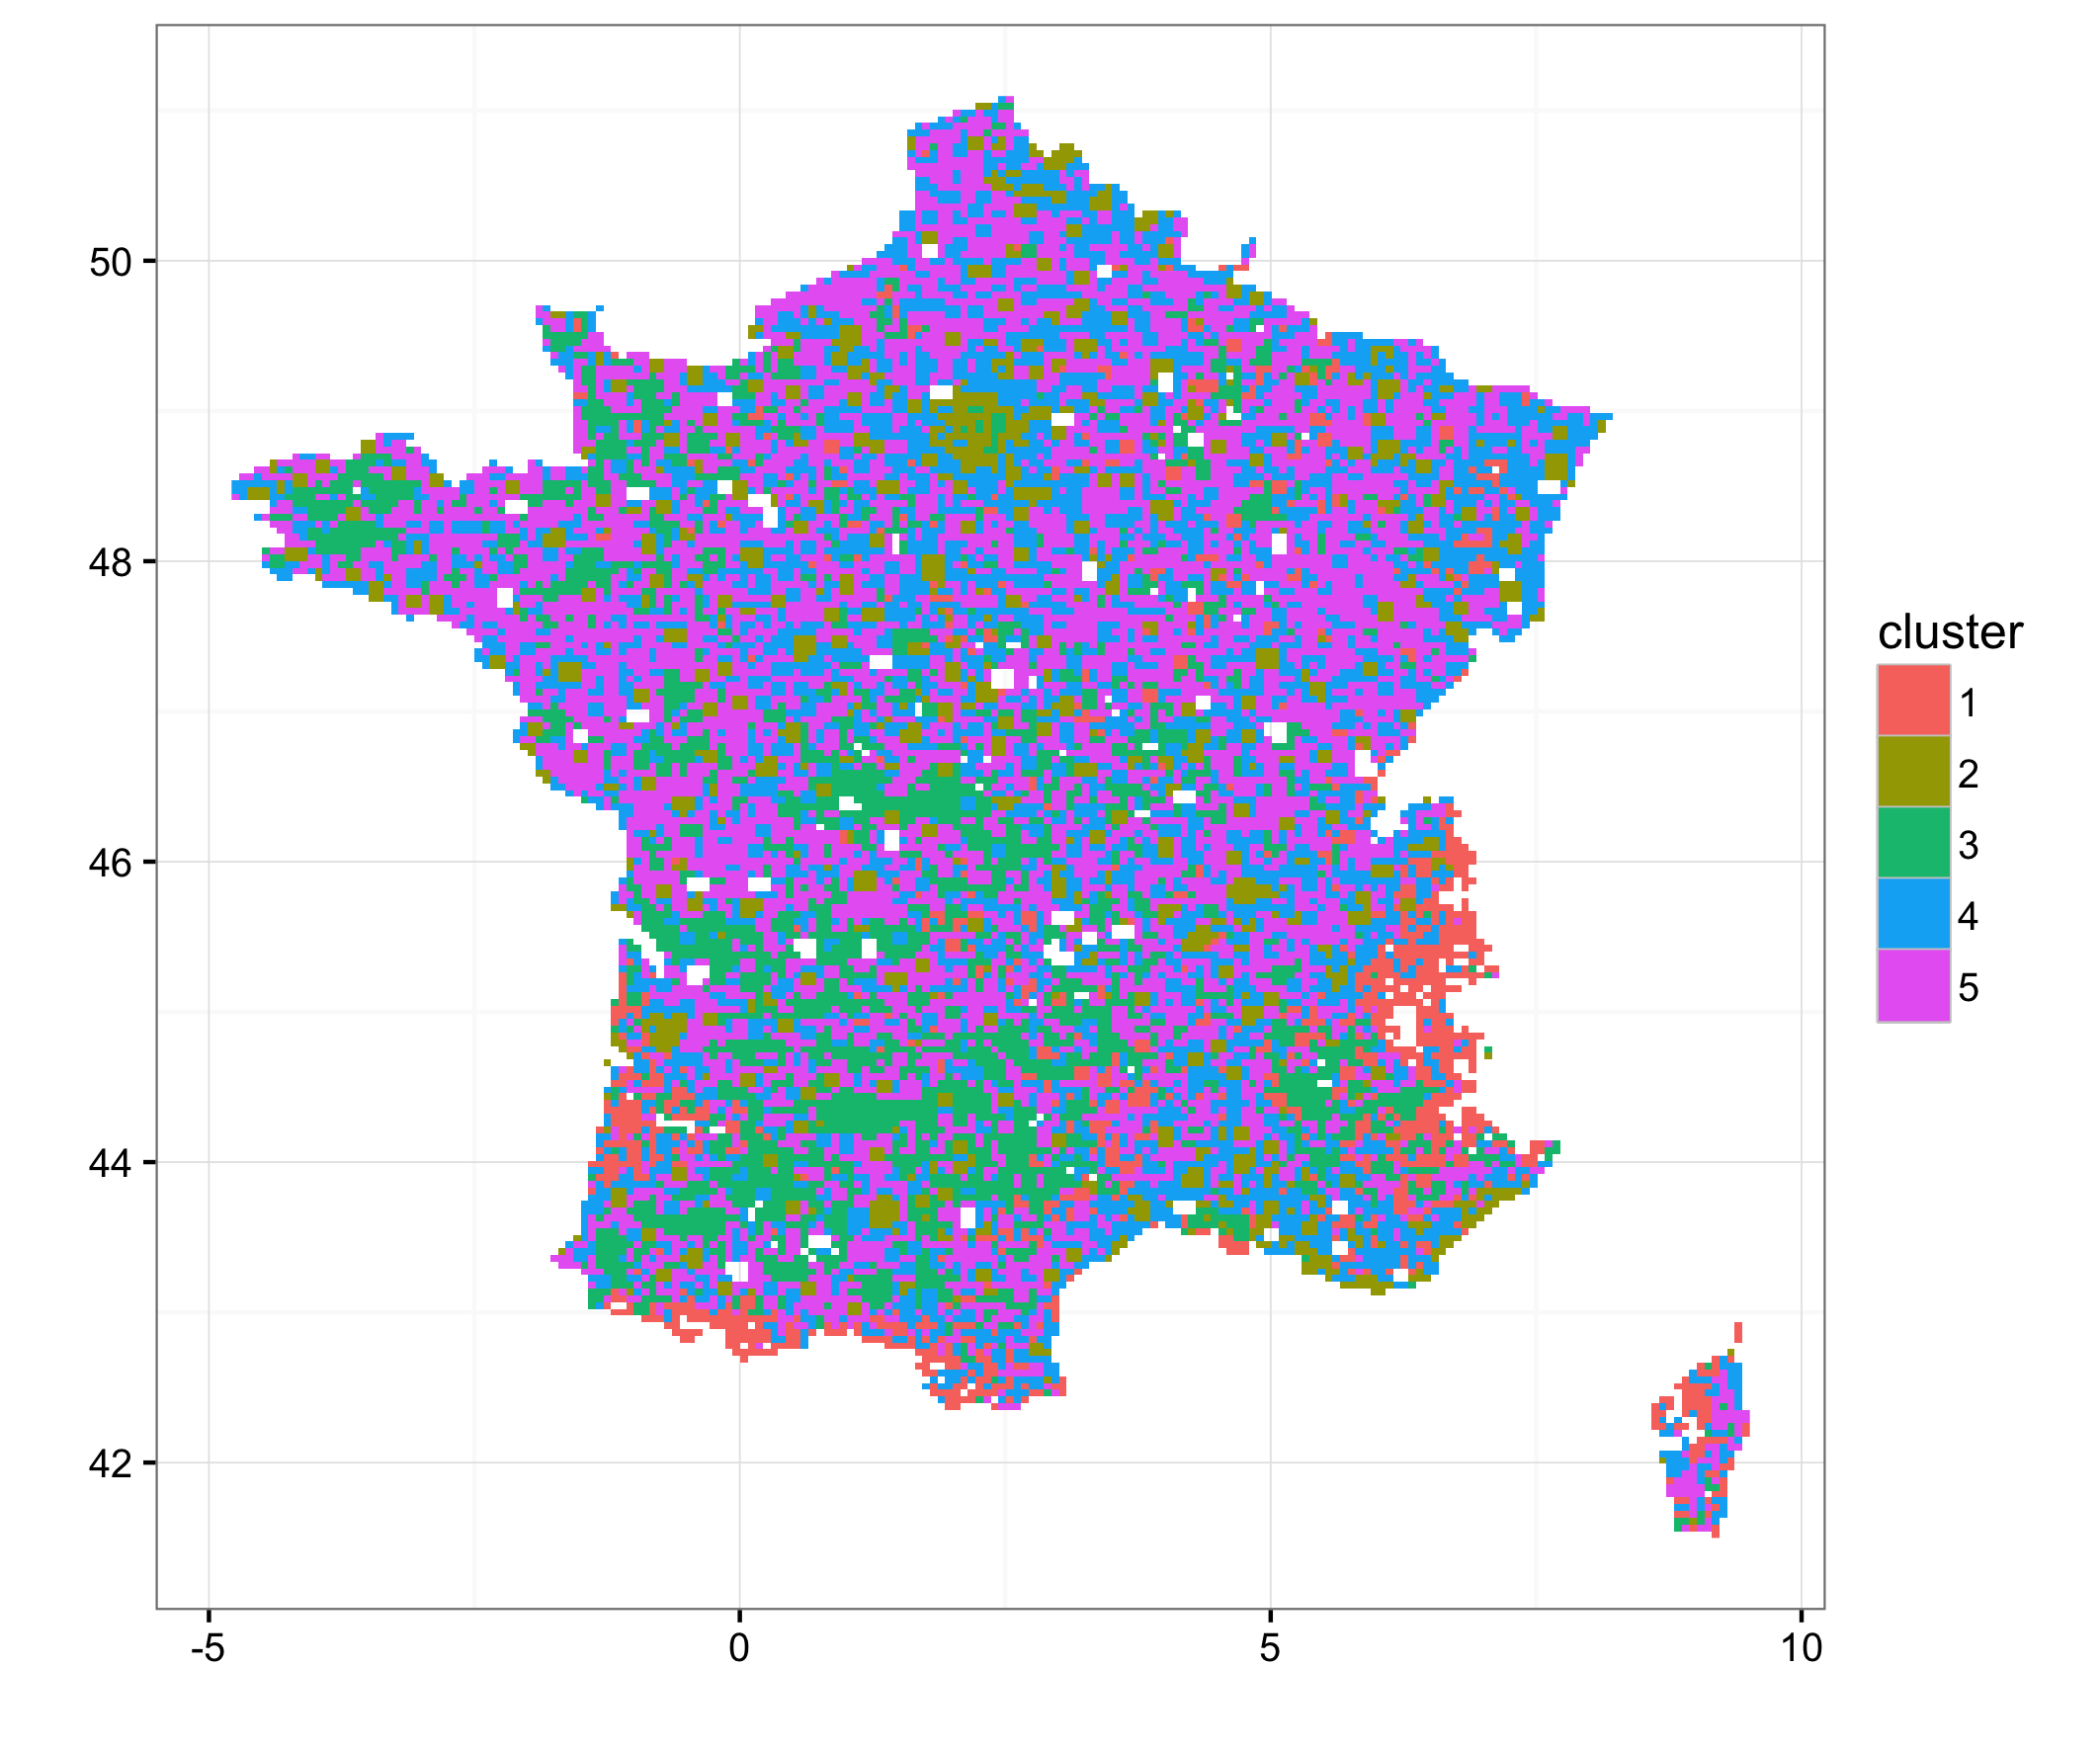
\includegraphics[width=0.49\textwidth]{figures/cluster_map_k5_morpho}
\caption[Empirical values of morphological indicators][Distribution spatiale des morphologies]{\textbf{Empirical values of morphological indicators.} \textit{(Top four maps)} Spatial distribution of the morphological indicators for France. Scale color discretization is done using quantiles to ease map readability. \textit{(Bottom Left)} Projection of morphological values on the two first components on a Principal Component analysis. Color gives cluster in an unsupervised classification (see text). \textit{(Bottom right)} Spatial distribution of clusters.}{\textbf{Valeurs empiriques de indicateurs morphologiques.} \textit{(Quatre cartes du haut)} Distribution spatiale des indicateurs morphologiques pour la France. La détermination de l'échelle de couleur est faite par quantiles pour faciliter la lecture des cartes. \textit{(Bas gauche)} Projection des valeurs morphologiques sur les deux premières composantes d'une analyse en composantes principales. La couleur donne le cluster dans une classification non supervisée (voir texte). \textit{(Bas droite)} Distribution spatiale des clusters.}
\label{fig:staticcorrelations:empirical}
\end{figure}
%%%%%%%%%%%%%%%%%%%%%%%%



\bpar{
We compute the morphological measures given above on real urban density data, using the population density grid of the European Union at 100m resolution provided openly by Eurostat~\cite{eurostat}. The choice of the resolution, the spatial range, and the shape of the window on which indicators are computed, is made according to the thematic specifications given before. We consider 50km wide square windows to be in accordance with the expected spatial range of one model instance. As it also does not make sense to have a too detailed resolution because of data quality, we take $N=100$ and aggregate the initial raster data at a 500m resolution to meet this size on real windows. To have a rather continuous distribution of indicators in space, we overlap windows by setting an offset of 10km between each, what also somehow rules out the question of window shape bias by the ``continuity'' of values. We tested the sensitivity to window size by computing samples with 30km and 100km window sizes and obtained rather similar spatial distributions. We show in Fig.~\ref{fig:staticcorrelations:empirical} maps giving values of indicators for France only to ease maps readability. The first striking feature is the diversity of morphological patterns across the full territory. The auto-correlation is naturally high in Metropolitan areas, with the Parisian surroundings clearly detached. When looking at other indicators, it is interesting to denote regional regimes: rural areas have much less hierarchy in the South than in the North, whereas the average distance is rather uniformly distributed except for mountain areas. Regions of very high entropy are observed in the Center and South-West. To have a better insight into morphological regimes, we use unsupervised classification with a simple k-means algorithm, for which the number of clusters $k=5$ witnesses a transition in inter-cluster variance. The split between classes is plotted in Fig.~\ref{fig:empirical}, bottom-left panel, where we show measures projected on the two first components of a Principal Component Analysis (explaining 71\% of variance). The map of morphological classes confirms a North-South opposition in a background rural regime (clear green against blue), the existence of mountainous (red) and metropolitan (dark green) regimes. Such a variety of settlements forms will be the target for the model.
}{
Nous calculons les mesures morphologiques données ci-dessus sur des données réelles de densité, en utilisant la grille de population de l'Union Européenne à la résolution de 100m fournie de manière ouverte par Eurostat~\cite{eurostat}. Cette base a certains défauts de précision qui ont été reconnus~\cite{bretagnolle2016ville} mais nous agrégerons les données à un niveau suffisant pour les éviter. Le choix de la résolution, de la portée spatiale, et de la forme de la fenêtre sur laquelle les indicateurs sont calculés, sont faits suivant les spécifications thématiques précédentes. Nous considérons des fenêtres carrées de largeur 50km, ce qui permet de plus d'être en accord avec l'ontologie du modèle de morphogenèse que l'on développera en~\ref{sec:densitygeneration}. Comme cela ne fait pas sens d'avoir une résolution trop détaillée à cause de la qualité des données, nous agrégeons les données raster initiales à une résolution de 500m pour avoir des fenêtres de taille $N=100$. Pour obtenir une distribution des indicateurs relativement continue dans l'espace, nous superposons les fenêtres en posant un décalage de 10km entre chaque, ce qui d'une certaine façon résout le problème du biais de la forme de la fenêtre par la ``continuité'' des valeurs. Nous avons testé la sensibilité à la taille de la fenêtre en calculant des échantillons avec des tailles de 30km et 100km et avons obtenu des distributions spatiales assez similaires. L'implémentation des indicateurs doit être faite avec attention, puisque les complexités computationnelles peuvent atteindre $O(N^4)$ pour l'indice de Moran par exemple: nous utilisons les implémentations en \texttt{R} de la convolution par Transformée de Fourier Rapide. Nous montrons en Fig.~\ref{fig:staticcorrelations:empirical} des cartes donnant les valeurs des indicateurs, pour la France seulement afin de permettre une lisibilité. Pour avoir une idée des valeurs typiques de chacun des indicateurs, on pourra se référer aux distributions empiriques données en Appendice~\ref{app:sec:staticcorrelations}. La première caractéristique frappante est la diversité des motifs morphologiques au travers de l'ensemble du territoire. L'auto-correlation est relativement haute dans les zones métropolitaines, avec les environs de Paris qui se détachent clairement. Lorsqu'on s'intéresse aux autres indicateurs, il est intéressant de constater des régimes régionaux: les zones rurales ont beaucoup moins de hiérarchie dans le Sud que dans le Nord, tandis que la distance moyenne est plutôt distribuée uniformément sauf dans les zones montagneuses. Des régions à très forte entropie sont observées dans le centre et le Sud-ouest. Pour avoir une meilleure compréhension des régimes morphologiques, nous utilisons une classification non-supervisée avec un algorithme des k-means simple, pour lequel le nombre de clusters $k=5$ induit une transition dans la variance inter-cluster. La séparation entre les classes est montrée en~\ref{fig:staticcorrelations:empirical}, panneau bas gauche, où nous représentons les mesures projetées sur les deux premières composantes d'une Analyse en Composantes Principales (expliquant 71\% de la variance, ce qui est relativement conséquent). La carte des classes morphologiques confirme une opposition Nord-Sud dans le régime rural de fond (vert clair contre bleu), l'existence d'un régime de montagne (rouge) et d'un régime métropolitain (vert sombre). Une telle variété d'établissements sera l'un des objectifs du modèle en~\ref{sec:densitygeneration}.
}






%%%%%%%%%%%%%%%%%%
\subsection{Network Measures}{Mesures de Réseau}


\bpar{
We consider network aggregated indicators as a way to characterize transportation network properties on a given territory, the same way morphological indicators yielded information on urban structure. We propose to compute some simple indicators on same extents as for morphology, to be able to explore relations between these static measures. Static network analysis has been extensively documented in the literature, see for example \cite{louf2014typology} for a cross-sectional study of cities or \cite{2015arXiv151201268L} for exploration of new measures for the road network.
}{
Nous considérons d'autre part les mesures agrégées de réseau comme un moyen de caractériser les propriétés des réseaux de transport sur un territoire donné, de la même façon que les indicateurs morphologiques informent sur la structure urbaine. Nous proposons de calculer des indicateurs simples sur des étendues spatiales similaires à la morphologie, pour être en mesure d'explorer les relations entre ces mesures statiques. L'analyse statique de réseau a été intensément documentée dans la littérature, voir par example \cite{louf2014typology} pour une étude comparative des villes ou \cite{2015arXiv151201268L} pour l'exploration de nouvelles mesures pour le réseau de rues.
}


\subsubsection{Data preprocessing}{Pré-traitement des données}


\bpar{
We work here with the road network, which structure is finely conditioned to territorial configuration of population densities. Furthermore, data for present day road network is openly available through the OpenStreetMap project~\cite{openstreetmap}. Its quality was investigated for different countries such as England~\cite{haklay2010good} and France~\cite{girres2010quality}. It was found to be of a quality equivalent to official surveys for the primary road network.
}{
Nous travaillons ici avec le réseau de rues, dont la structure est finement conditionnée aux configurations territoriales des densités de population. De plus, les données du réseau de routes actuel est disponible ouvertement par l'intermédiaire du projet OpenStreetMap (OSM)~\cite{openstreetmap}. Sa qualité a été étudiée pour différents pays comme l'Angleterre~\cite{haklay2010good} et la France~\cite{girres2010quality}. Il a été établi pour ces pays une qualité équivalente aux données officielles pour le réseau de rues primaire.
}


\bpar{
Although \cite{zheng2014assessing} underlined a quick acceleration of OpenStreetMap road data completeness and accuracy, its use for computation of network indicators may be questioned. \cite{zhang2015density} highlights four regimes of data quality, partitioning China into regions among which qualitative behavior of OSM data varies. We underline that the results will be more valid on the regions where the quality is the highest, i.e. with high density and high diversity. For density data, we use the gridded population data from~\cite{fu1km}.
}{

}



\bpar{
From the primary road segments, we compute the topological road network for all studied areas, at 100m granularity scale to be used consistently with the population grid. The OSM data is imported into \texttt{pgsql} using \texttt{osmosis}, is then aggregated at fixed granularity, and the resulting topological network is finally simplified with a split/merge algorithm.
}{
Pour les segments de rue primaires, nous calculons le réseau topologique pour l'ensemble des zones étudiées, à une granularité de 100m pour pouvoir être utilisé de manière cohérente avec les grilles de population. Les données OSM sont importées dans \texttt{pgsql} en utilisant \texttt{osmosis}~\cite{osmosis}, est ensuite agrégé à la granularité fixe, et le réseau topologique résultant est finalement simplifié avec un algorithme split/merge.
}


   \textit{$\simeq 44\cdot 10^6$ links in initial OSM db, $\simeq 61\cdot 10^6$ in first simplified layer, $\simeq 21\cdot 10^6$ in final database}



For a given dataset corresponding to a subset of the overall road network, it is necessary to simplify network structure by spatial aggregation as initial data presents very detailed features and thus a very large numbers of nodes ($\simeq 10^10$ for Europe dataset). \comment{(Florent) c'est un peu confus, tu devrais d'abord dire : ce que tu as, les pb que ça pose, comment les résoudre}
 Such a level of precision is not needed in our study since density data is already aggregated at 500m resolution. It is possible to drastically reduce network size by spatial aggregation of nodes and link replacements. The detailed algorithm and implementation are detailed in Supplementary material~\ref{app:sec:staticcorrelations}.




\subsubsection{Indicators}{Indicateurs}


\bpar{
These indicators are used to capture a rough picture of the structure. Refined work at smaller scales (intra-urban road network) and with more elaborated measures that allow to differentiate more precisely local form, was recently done by Lagesse in~\cite{2015arXiv151201268L}.
}{
Nous introduisons des indicateurs pour avoir une idée large de la forme du réseau. Un travail plus élaboré à des échelles plus fines (réseau de rues intra-urbain) et avec des mesures plus raffinées permettant de discriminer localement des formes typiques, a été récemment mené par \noun{Lagesse} dans~\cite{2015arXiv151201268L}. Dans notre cas, nous utilisons une batterie d'indicateurs pour capturer le maximum de dimensions des propriétés des réseaux, plus ou moins liées à l'utilisation de ceux-ci
}


\bpar{
Network macroscopic structure is summarized by the following set of indicators, after the simplifications and reductions done in the previous step. Assuming network given by $N=(V,E)$, nodes spatial positions $\vec{x}(V)$ and edges \emph{effective distances} $d(E)$ taking into account impedances and real distances (to include basically network hierarchy), we have indicators:
}{
Dans notre cas, nous résumons la structure macroscopique du réseau par un jeu fixé d'indicateurs, calculés sur les réseau topologiques obtenus par les étapes précédentes de simplification. Notant le réseau $N=(V,E)$, les noeuds ayant les positions spatiales $\vec{x}(V)$ et les liens des \emph{distances effectives} $d(E)$ qui prennent en compte les impédances et les distance réelle (pour inclure la hiérarchie primaire du réseau), nous avons les indicateurs :
}



\begin{itemize}
\item connectivity
\item degree distribution
\item centrality, taken as normalized mean \emph{betweenness-centrality}
\item average path length
\item network diameter
\item mean network speed
\end{itemize}

L'accessibilité est bien considérée comme un indicateur de réseau, puisque son calcul implique d'attribuer des poids aux noeuds par un population correspondante, et revient ensuite à un temps de trajet moyen pondéré. Cet indicateur est intéressant car à l'interface entre forme urbaine et forme du réseau, puisque la distribution de population sur les noeuds est prise en compte. On verra que celle-ci est fortement corrélée au même non-pondéré ($\rho = 0.86$ pour l'ensemble de la Chine par exemple).



\subsubsection{Network Shape and Resilience}{Forme de Réseau et Résilience}

L'idée fondamentale motivant le calcul d'indicateurs de réseau est d'obtenir une réduction de dimension drastique, s'il est possible d'associer certains ``types'' de réseau à des valeurs typiques d'indicateurs. On est très loin d'une connaissance fine de typologies qui associeraient propriétés topologiques, dynamiques et processus de génération du réseau, le tout dans des typologies. De même que lier ces propriétés à des caractéristiques dérivées, comme la résilience qui est une propriété aux définitions diverses pour laquelle~\cite{Gao:2016ty} introduit une approche par la sensibilité des processus dynamiques. Afin d'illustrer d'une part la difficulté de caractériser les réseaux et d'autre part les potentialités offertes par notre base de données, nous développons en Appendice~\ref{app:sec:staticcorrelations} une courte analyse des propriétés de résilience au sens de~\cite{ash2007optimizing} pour des réseaux typiques.



\subsubsection{Results}{Résultats}


\bpar{}{
Les indicateurs de réseau ont été calculés sur les mêmes zones que les indicateurs de forme urbaine, pour pouvoir les mettre en correspondance directe et calculer les correlations par la suite.

}




%%%%%%%%%%%%%%%%%%%%%%%%
\begin{figure}
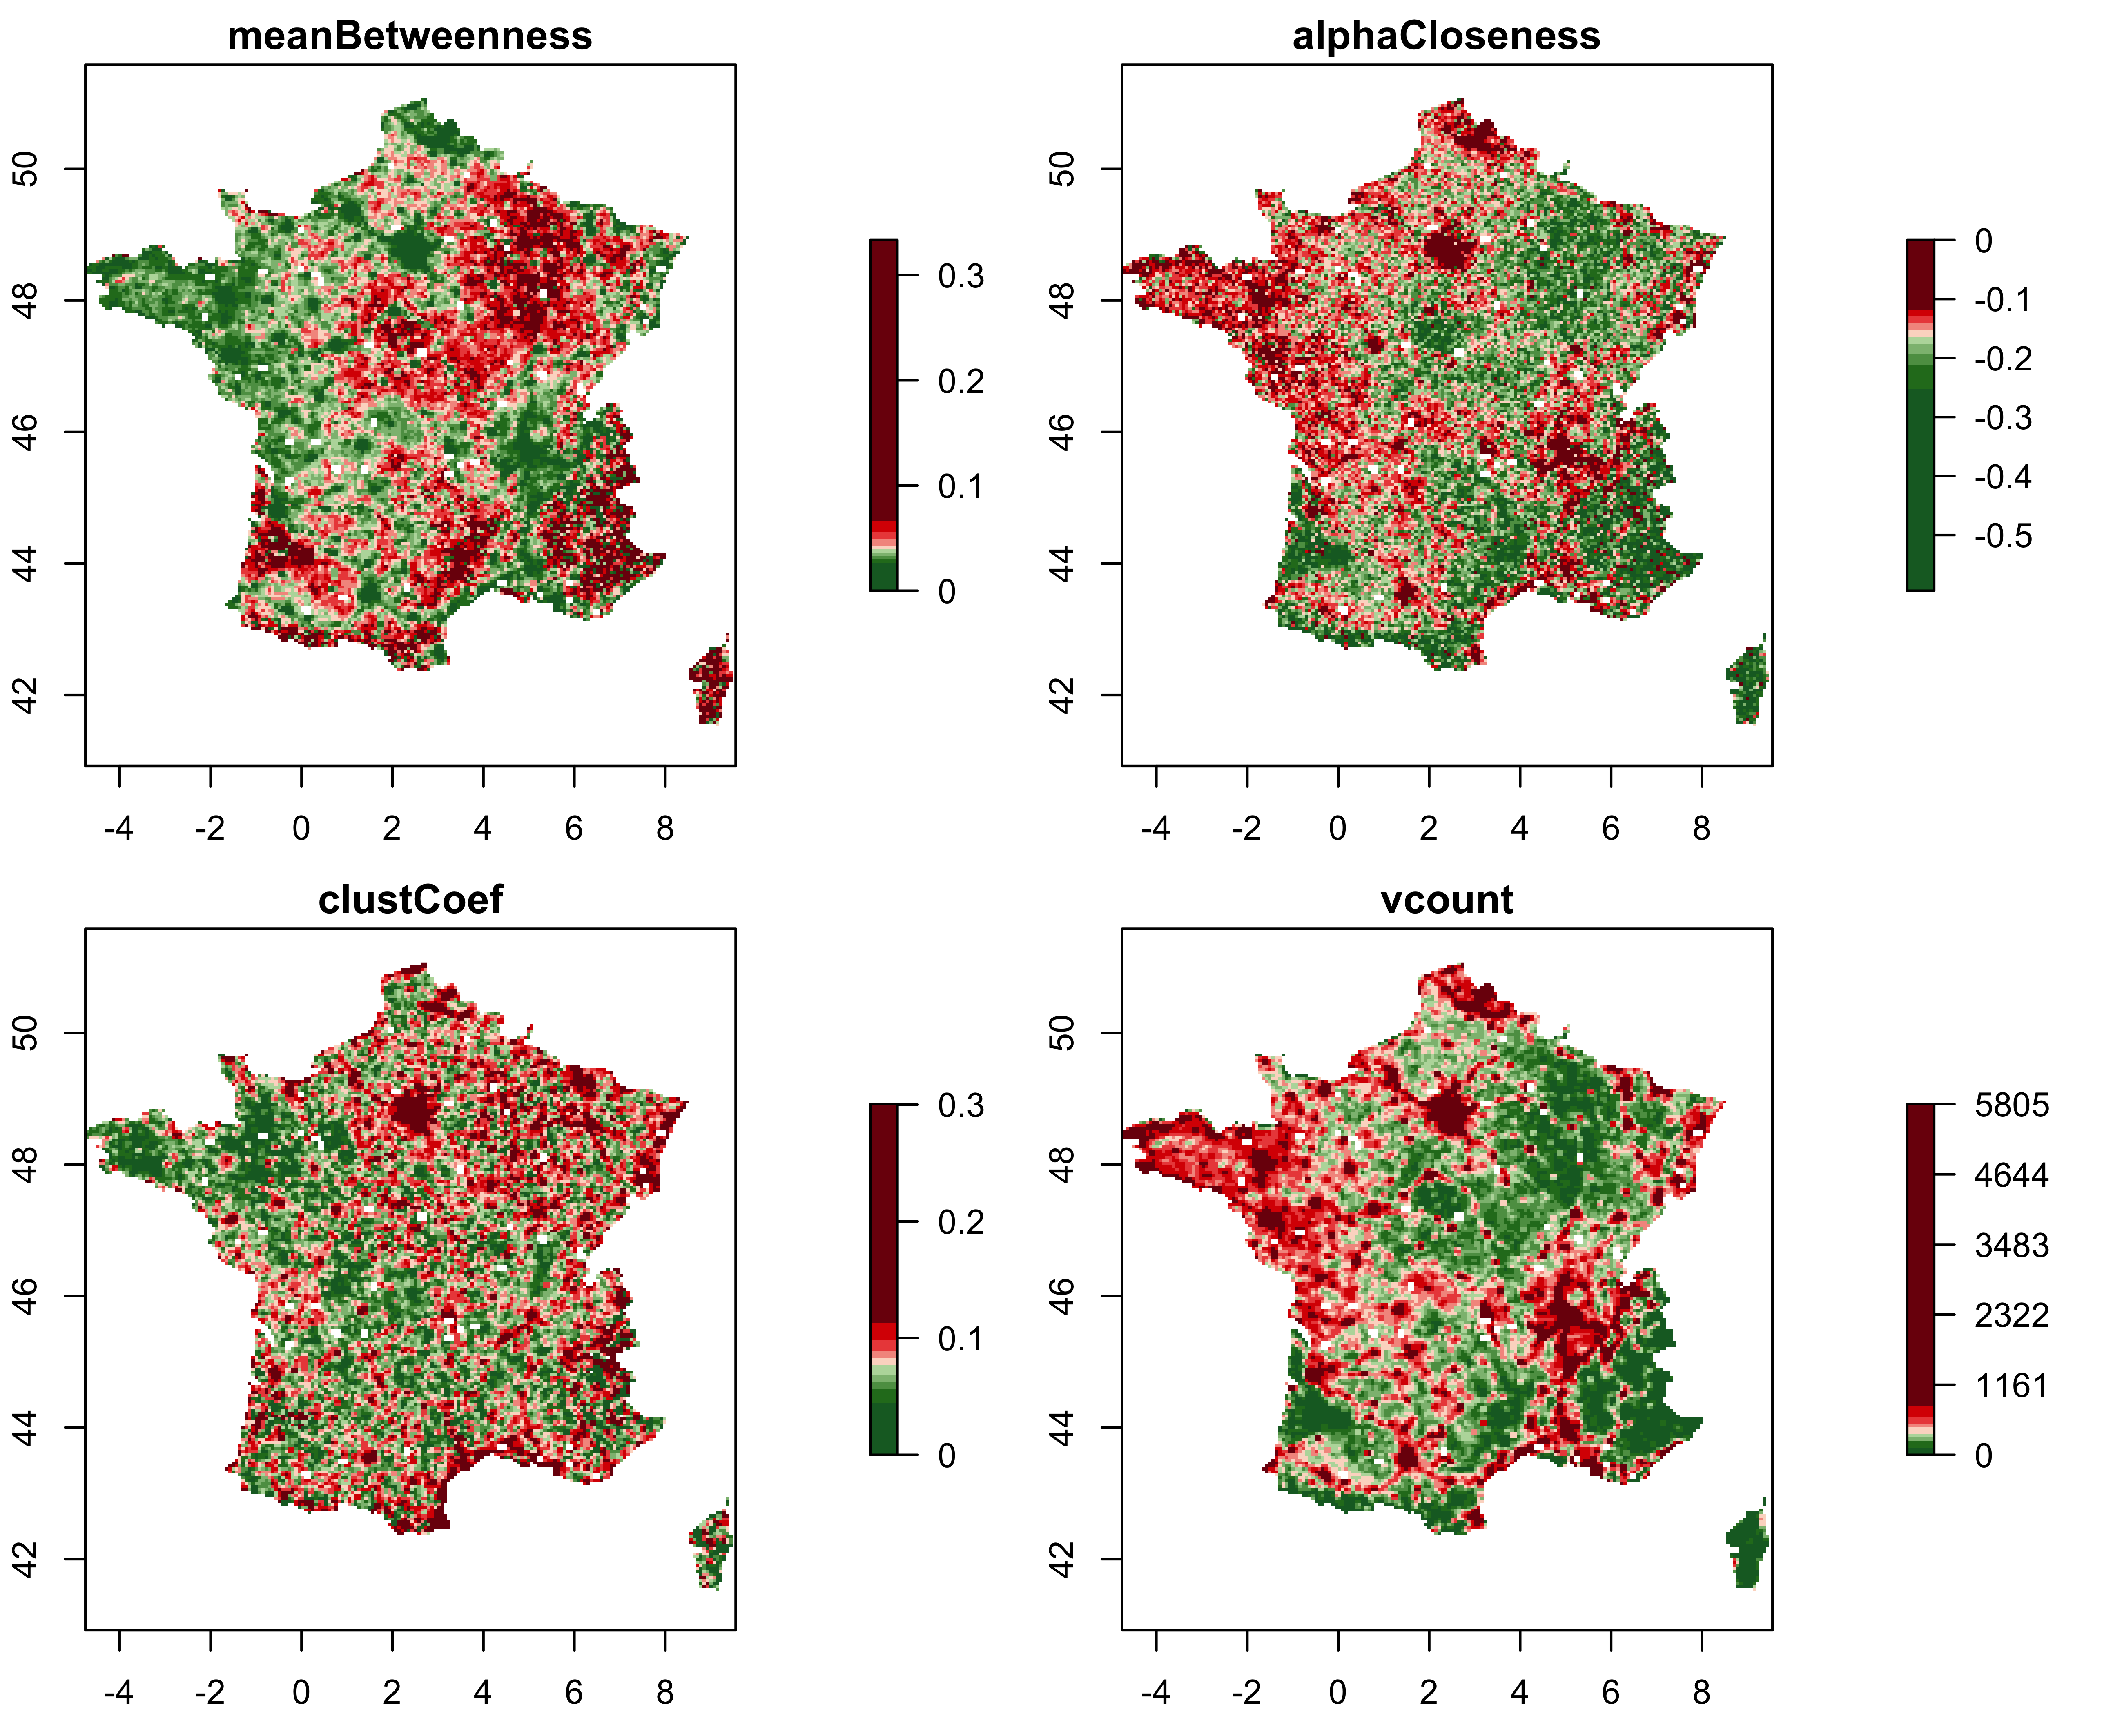
\includegraphics[width=\linewidth]{Figures/StaticCorrelations/FR_indics_network_selected_2_discrquantiles}
\caption[Empirical values of network indicators][Distribution spatiale des indicateur de réseau]{\textbf{Empirical values of network indicators.}}{\textbf{Distribution spatiale des indicateur de réseau.}}
\label{fig:staticcorrs:network}
\end{figure}
%%%%%%%%%%%%%%%%%%%%%%%%





%%%%%%%%%%%%%%%%%%
\subsection{Effective static correlations}{Correlations Statiques Effectives et Non-stationnarité}


%%%%%%%%%%%%%%%%%%
\subsubsection{Correlations}{Corrélations}

% short overview of overall correlations and effective dimensions






%%%%%%%%%%%%%%%%%%
\subsubsection{Spatial Correlations}{Corrélations spatiales}


Pour les correlations : zones de correlation pas trop grandes, carrés de base indicateurs plus petits : Computation of urban form indicators~\cite{le2015forme} and network indicators on $l_0=10km$ side square

Computation of spatial correlation on square areas of width $\delta\cdot l_0$ (with typically $\delta = 4, \ldots , 16$)


We clearly unveil the local spatial stationarity of processes.

% some maps
%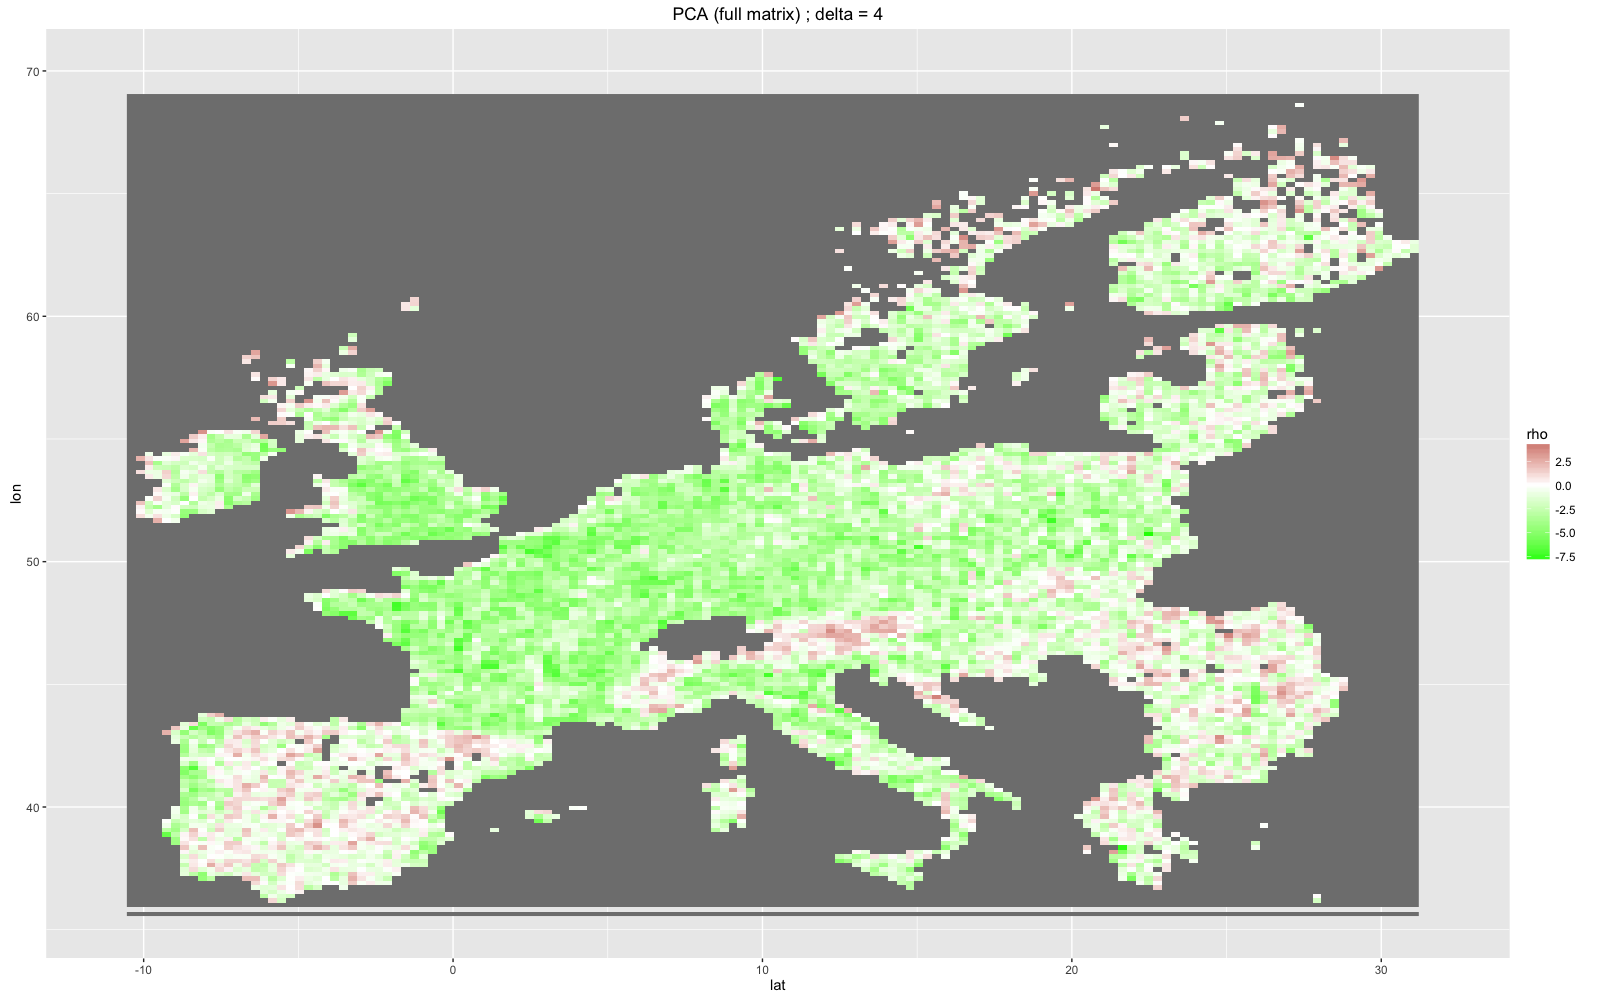
\includegraphics[width=\textwidth,height=0.7\textheight]{figures/corr_PCA_delta4}




\paragraph{Multi-scale Processes}{Nature multi-scalaire des processus}

% plots
%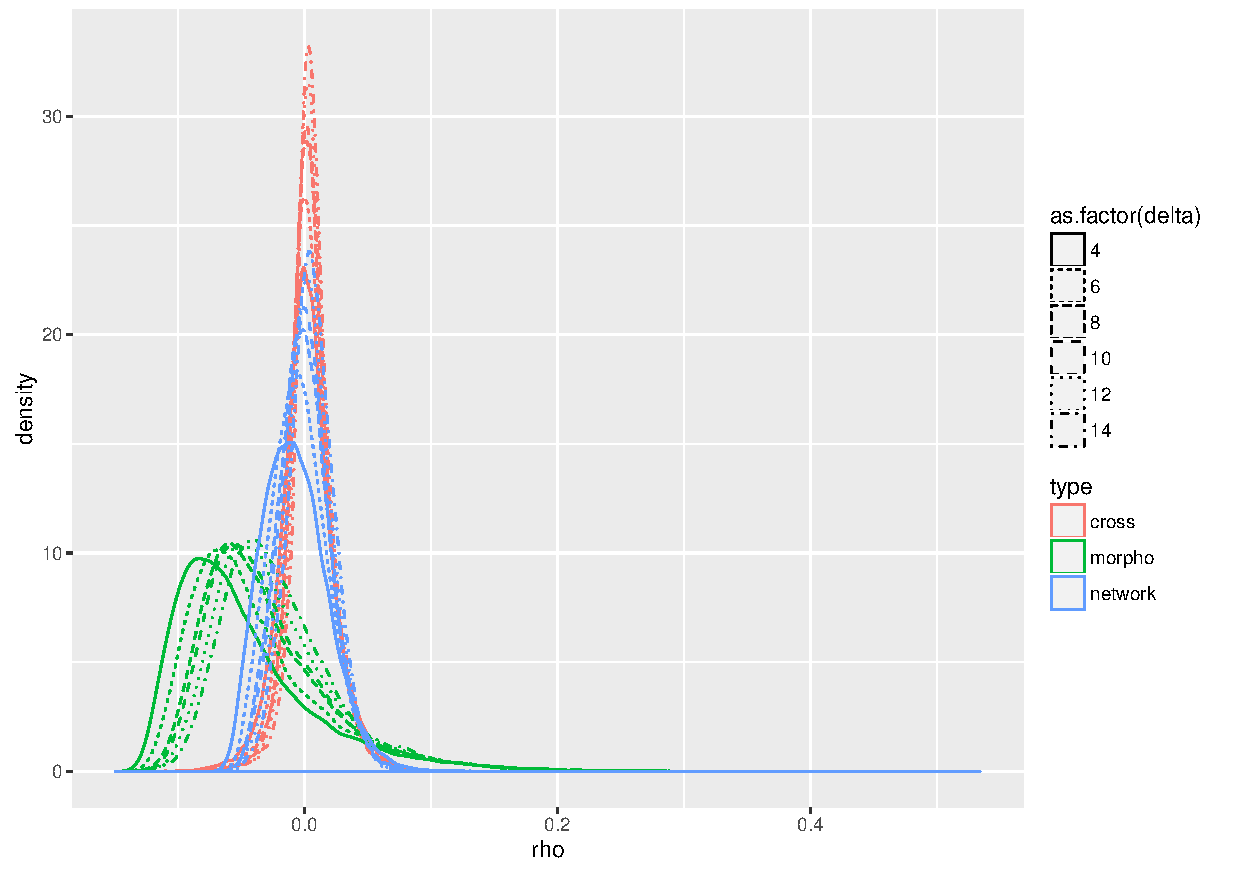
\includegraphics[width=0.33\textwidth]{figures/corrs-distrib_varyingdelta_bytype} % -> in supp material
%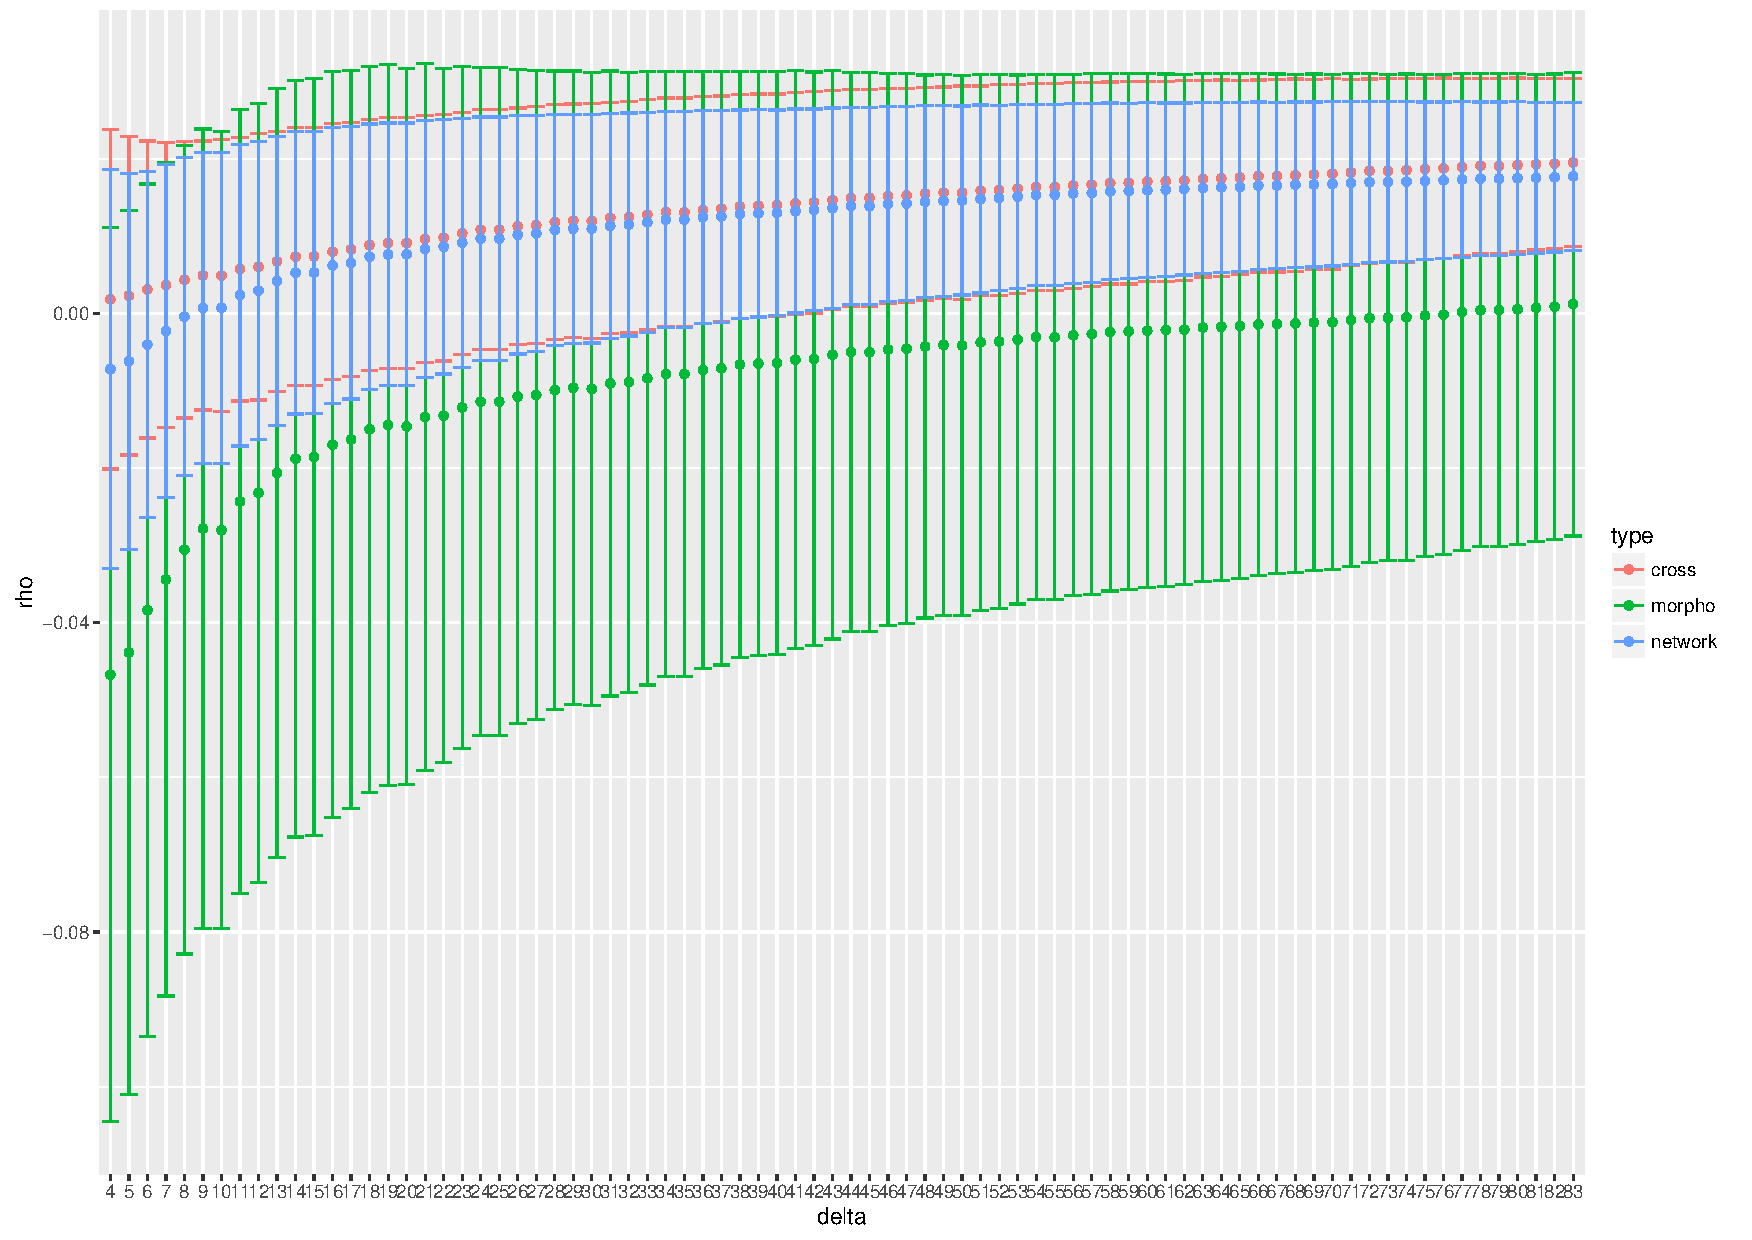
\includegraphics[width=0.5\textwidth]{figures/corrs-summary_varyingdelta_bytype_extended1}
%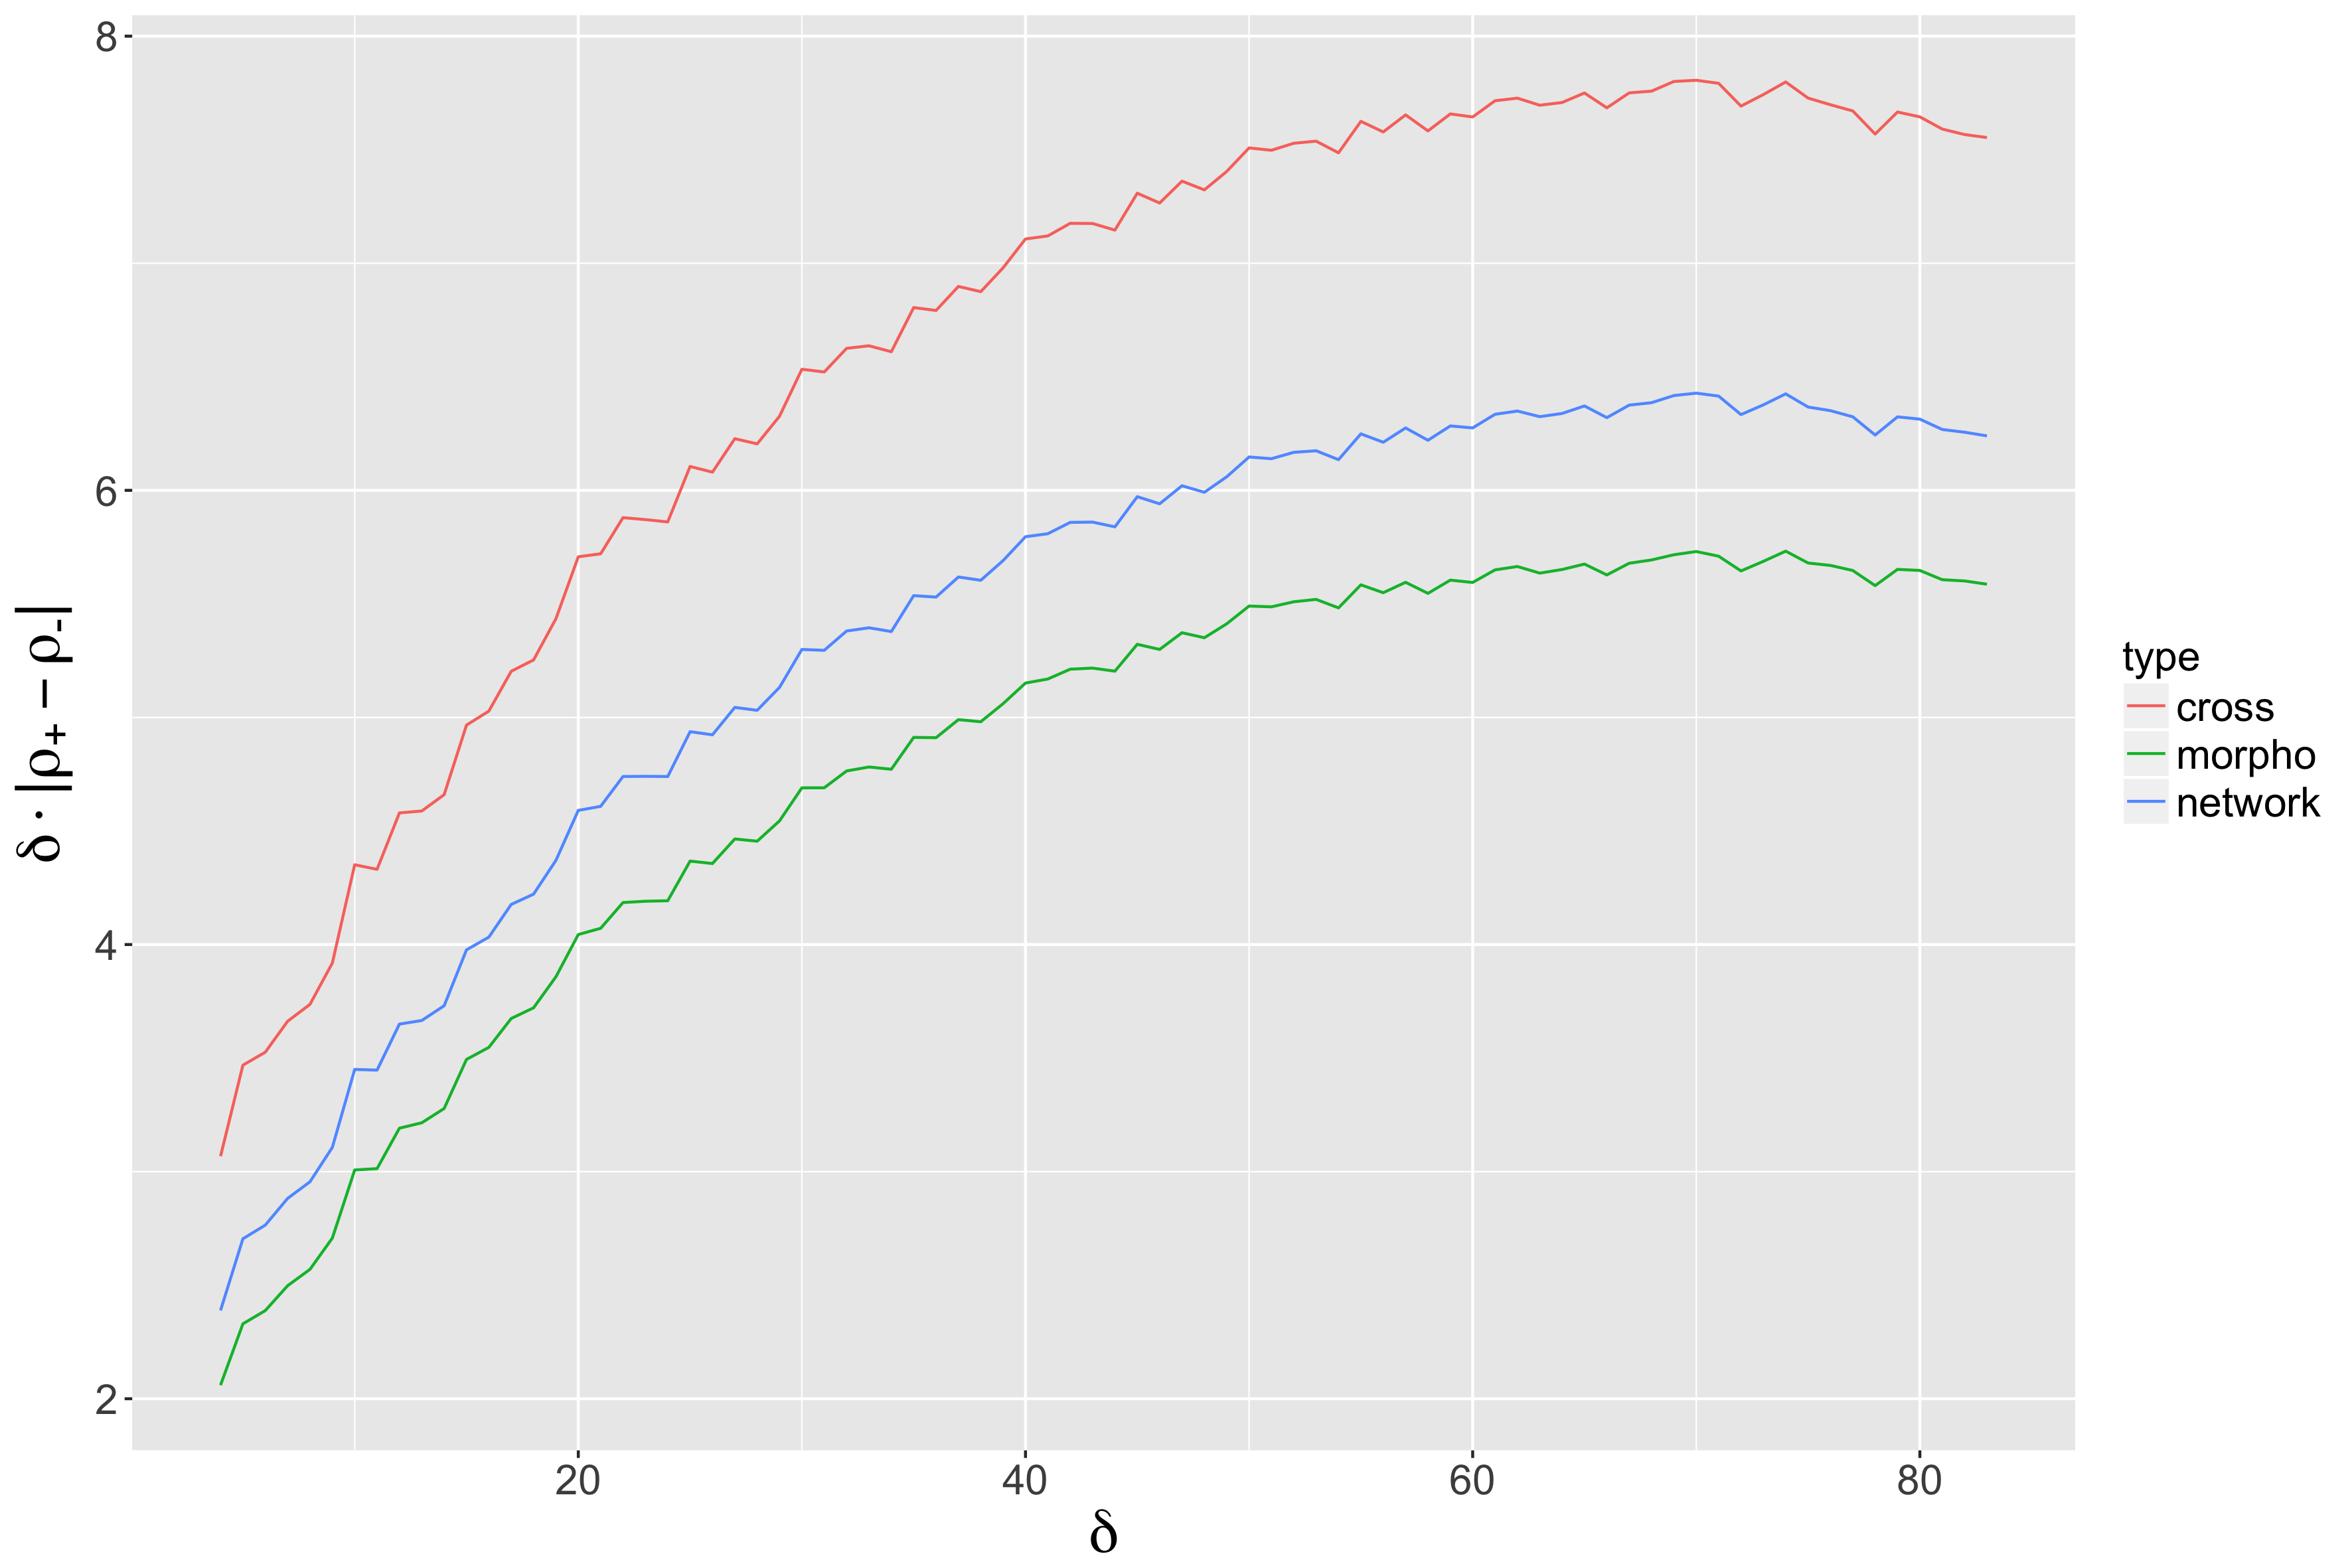
\includegraphics[width=0.5\textwidth]{figures/normalized_CI_delta}


On observe une variation significative des correlations moyennes en fonction de $\delta$

$\rightarrow$ Significant variation of mean correlation with $\delta$ (Left) and of normalized confidence interval (Right) given by $\left|\rho_+ - \rho_-\right|\cdot \delta$, as bounds theoretically vary as $\sqrt{N} \sim \sqrt{\delta^2}$ : implies multi-scalarity




We also compute the optimal bandwidth for a GWR PCA~\cite{harris2011geographically}

\cite{wheeler2007diagnostic} colinearity in GWR






%%%%%%%%%%%%%%%%%%
\subsubsection{Spatial non-stationarity and non-ergodicity}{Non-stationnarité spatiale et non-ergodicité}


\paragraph{Formalization}{Formalisation}

\bpar{
We propose to formalize our empirical findings

Let $Y_i\left[\vec{x},t\right]$ a spatio-temporal stochastic process. We showed it verifies empirically the following assumptions:
\begin{enumerate}
\item Local spatial autocorrelation is present and bounded by $l_{\rho}$ (in other words the processes are continuous in space) : at any $\vec{x}$ and $t$, $\left|\rho_{\norm{\Delta \vec{x}} < l_{\rho}}\left[Y_i (\vec{x}+\Delta \vec{x},t), Y_i (\vec{x},t) \right]\right| > 0$.
\medskip
\item Processes are locally parametrized : $Y_i = Y_i\left[\alpha_i\right]$, where $\alpha_i (\vec{x})$ varies with $l_{\alpha}$, with $l_{\alpha} \gg l_{\rho}$ and weakly locally stationary in space.
\medskip
%\item Spatial correlations between processes have a sense at an intermediate scale $l$ such that $l_{\alpha}\gg l \gg l_{\rho}$.
%\item Processes covariance stationarity times scale as $\sqrt{l}$.
%\item Local ergodicity is present at scale $l$ and dynamics are locally chaotic.
\item Processes are multi-scalar : since $\rho(\delta = \infty) > \rho (\delta = 0 )$, a necessary non-linear correction on processes spatial averages in correlation computation is present.
% add computation in supplementary materials / papers. -> later
\end{enumerate}
}{

}


\paragraph{On global non-ergodicity}{Sur la non-ergodicité globale}

Analytical Deductions

1. \textbf{Regimes of temporal correlations.} Let assume local ergodicity in $\vec{x}_0$ at scale $\delta \cdot l_0$ (reasonable with urban growth and network extension in recent times). The Ergodic theorem implies that $\exists \mathcal{T}$ such that

\[<Y_i (t) >_{\norm{\vec{x}-\vec{x}_0} < \delta\cdot l_0} = <Y_i (\vec{x}_0)>_{t\in \mathcal{T}}\] 

With spatial stationarity, $<Y_i>_{\vec{x}_0}=<Y_i>_{\vec{x}_1}$, thus $\mathcal{T}$ must be constant to be invariant by translation. By contraposition and (2), processes have different dynamical characteristics.
% if translate in a given direction, looses a small part, must be compensated by the area translated by delta (overlap), thus must be constant.


2. \textbf{Global non-ergodicity.} Let $X_k$ a partition of space into local areas. We have $<\cdot>_x = \sum_k w_k <\cdot>_{x_k} =_{(1)} \sum_k w_k <\cdot>_{\mathcal{T}_k} $. On the other hand, global ergodicity would give $<\cdot>_t = <\cdot>_{\mathcal{T}} = \sum_k w_k <\cdot>_{\mathcal{T}}$ and $\sum_k w_k \left(<\cdot>_{\mathcal{T}} - <\cdot>_{\mathcal{T}_k}\right) = 0$. Being true on each subset implies $\mathcal{T}=\mathcal{T}_k$, what contradicts (1).





Case study : implications
% thematic conclusion of the case study on ergodicity

Assuming local ergodicity, spatial local stationarity implies and temporal local stationarity. Spatial non-stationarity \textbf{at the second order}$\implies$ temporal scale variations $\implies$ non-ergodicity


$\rightarrow$ We show the regional nature of network-territories interactions, in particular the non-ergodicity of urban systems on \textbf{the interaction these components}


$\rightarrow$ No direct results on time dynamics, but indirect : spatio-temporal processes do not have same speed and react/diffuse differently








%%%%%%%%%%%%%%%%%%
\subsubsection{Discussion}{Discussion}


\paragraph{Universality}{Universalité}

\bpar{
In \cite{10.1371/journal.pone.0107042} density grids for other countries across the world are provided\footnote{available at \url{http://www.worldpop.org.uk/}}. The analysis may be repeated to other regions of the world, to compare the correlation regimes and test if urban system properties stay the same. We can expect different regimes for the United States compared to Europe for example, but the discrepancy needs still to be investigated~\cite{bretagnolle2010comparer}.
}{
Des grilles de densité de population existent pour l'ensemble des régions du monde, comme par exemple celles fournies par~\cite{10.1371/journal.pone.0107042}\footnote{disponibles à \url{http://www.worldpop.org.uk/}}. L'analyse peut être répétée pour d'autres régions, pour comparer les régimes de corrélations et tester si les propriétés des systèmes urbains restent les mêmes, en gardant à l'esprit les difficultés liées aux différences de qualité dans les données. On peut s'attendre à des régimes très différents pour les Etats-Unis en comparaison à l'Europe par exemple~\cite{bretagnolle2010comparer}, mais la différence se doit d'être étudiée quantitativement.
}



\paragraph{Further Developments}{Développements}

$\rightarrow$ Still points to explore :
\begin{itemize}
\item variable correlations areas (size and shape in space)
\item same work on cities population/train network data, which are also dynamical databases : extrapolation of ergodicity parameters ?
\item correlations of returns : link between $\rho\left[\Delta_t Y\right]$ and $\rho\left[\Delta_x Y\right]$ (more difficult : if pure local ergodicity, $\exists$ a permutation making the correspondance) % may be difficult to identify 
\item Link between $\Delta_{\delta}\rho (\delta)$ and process derivatives ?
\end{itemize}









\stars




